% Created 2023-06-24 Sat 18:37
% Intended LaTeX compiler: pdflatex
\documentclass[10pt,leftblank,twoside]{mitthesis}
\usepackage[utf8]{inputenc}
\usepackage[T1]{fontenc}
\usepackage{graphicx}
\usepackage{longtable}
\usepackage{wrapfig}
\usepackage{rotating}
\usepackage[normalem]{ulem}
\usepackage{amsmath}
\usepackage{amssymb}
\usepackage{capt-of}
\usepackage{hyperref}
\usepackage{minted}
\usepackage{lgrind}
\usepackage{cmap}
\usepackage[T1]{fontenc}
\pagestyle{plain}
\usepackage{algorithm2e}
\usepackage{amsthm}
\usepackage{amsmath}
\usepackage{graphicx}
\usepackage{mathtools}
\usepackage{minted}
\def\all{all}
\ifx\files\all \typeout{Including all files.} \else
\date{}
\title{Main SM Thesis Cover Abstract Ch1 Introduction Problem Statement Approach Technical VDC Technical Scheduling Technical Distributed Technical Robustness Evaluation Discussion POSTNU to VDC Comparison}
\hypersetup{
 pdfauthor={Cameron W Pittman},
 pdftitle={Main SM Thesis Cover Abstract Ch1 Introduction Problem Statement Approach Technical VDC Technical Scheduling Technical Distributed Technical Robustness Evaluation Discussion POSTNU to VDC Comparison},
 pdfkeywords={},
 pdfsubject={},
 pdfcreator={Emacs 28.2 (Org mode 9.6)}, 
 pdflang={English}}
\makeatletter
\newcommand{\citeprocitem}[2]{\hyper@linkstart{cite}{citeproc_bib_item_#1}#2\hyper@linkend}
\makeatother

\usepackage[notquote]{hanging}
\begin{document}

%% The documentclass options along with the pagestyle can be used to generate
%% a technical report, a draft copy, or a regular thesis. You may need to
%% re-specify the pagestyle after you \include cover.tex. For more
%% information, see the first few lines of mitthesis.cls.
%%
%\documentclass[12pt,vi,twoside]{mitthesis}
%%
%%  If you want your thesis copyright to you instead of MIT, use the
%%  ``vi'' option, as above.
%%
%\documentclass[12pt,twoside,leftblank]{mitthesis}
%%
%% If you want blank pages before new chapters to be labelled ``This
%% Page Intentionally Left Blank'', use the ``leftblank'' option, as
%% above.

%% These have been added at the request of the MIT Libraries, because
%% some PDF conversions mess up the ligatures.  -LB, 1/22/2014
%% This bit allows you to either specify only the files which you wish to
%% process, or `all' to process all files which you \include.
%% Krishna Sethuraman (1990).

%\typein [\files]{Enter file names to process, (chap1,chap2 ...), or `all' to process all files:}
%\typeout{Including only \files.} \includeonly{\files} \fi

\hypersetup{
  pdfauthor={Cameron W. Pittman},
  pdftitle={Distributed Multi-Agent Decision Making Under Uncertain Communication},
  pdfkeywords={},
  pdfsubject={},
  pdfcreator={Emacs 28.2 (Org mode 9.6)},
  pdflang={English}}

\usemintedstyle[lisp]{vs}

\graphicspath{{images/}}

\newcommand{\edge}[3]{#1 \xrightarrow{#3} #2}
\newcommand{\conedge}[3]{#1 \xRightarrow{#3} #2}
\newcommand{\gammabar}{\bar{\gamma}}
%\newcommand{\obs}{\texttt{obs}}
\newcommand{\obs}{\psi}
\newcommand{\assign}{\xi}

\newcommand{\finalversion}[1]{}

\newtheorem{theorem}{Theorem}[]
\newtheorem{corollary}{Corollary}[theorem]
\newtheorem{lemma}[theorem]{Lemma}

\newtheorem{transformation}{Transformation}

\theoremstyle{definition}
\newtheorem{defn}{Definition}

\theoremstyle{definition}
\newtheorem{example}{Example}

% NOTE:
% These templates make an effort to conform to the MIT Thesis specifications,
% however the specifications can change. We recommend that you verify the
% layout of your title page with your thesis advisor and/or the MIT
% Libraries before printing your final copy.

% FYI, the title and thesis need to be defined in the \hypersetup section in the main org file
\title{Distributed Multi-Agent Decision Making Under Uncertain Communication}
\author{Cameron W. Pittman}

% If you wish to list your previous degrees on the cover page, use the
% previous degrees command:
% You can use the \\ command to list multiple previous degrees
\prevdegrees{M.A., Belmont University (2011) \\
    B.A., Vanderbilt University (2009)}

\department{Department of Aeronautics and Astronautics}

% If the thesis is for two degrees simultaneously, list them both
% separated by \and like this:
% \degree{Doctor of Philosophy \and Master of Science}
\degree{Master of Science}

% As of the 2007-08 academic year, valid degree months are September,
% February, or June.  The default is June.
\degreemonth{June}
\degreeyear{2023}
\thesisdate{May 1, 2023}

%% By default, the thesis will be copyrighted to MIT.  If you need to copyright
%% the thesis to yourself, just specify the `vi' documentclass option.  If for
%% some reason you want to exactly specify the copyright notice text, you can
%% use the \copyrightnoticetext command.
%\copyrightnoticetext{\copyright IBM, 1990.  Do not open till Xmas.}

% If there is more than one supervisor, use the \supervisor command
% once for each.
\supervisor{Brian C. Williams}{Professor of Aeronautics and Astronautics, MIT}

% This is the department committee chairman, not the thesis committee
% chairman.  You should replace this with your Department's Committee
% Chairman.
\chairman{Jonathan How}{R.C Maclaurin Professor of Aeronautics and Astronautics, MIT \\
    Chair, Graduate Program Committee}

% Make the titlepage based on the above information.  If you need
% something special and can't use the standard form, you can specify
% the exact text of the titlepage yourself.  Put it in a titlepage
% environment and leave blank lines where you want vertical space.
% The spaces will be adjusted to fill the entire page.  The dotted
% lines for the signatures are made with the \signature command.
\maketitle


% The abstractpage environment sets up everything on the page except
% the text itself.  The title and other header material are put at the
% top of the page, and the supervisors are listed at the bottom.  A
% new page is begun both before and after.  Of course, an abstract may
% be more than one page itself.  If you need more control over the
% format of the page, you can use the abstract environment, which puts
% the word "Abstract" at the beginning and single spaces its text.

%% You can either \input (*not* \include) your abstract file, or you can put
%% the text of the abstract directly between the \begin{abstractpage} and
%% \end{abstractpage} commands.

% First copy: start a new page, and save the page number.
\cleardoublepage
% Uncomment the next line if you do NOT want a page number on your
% abstract and acknowledgments pages.
% \pagestyle{empty}
\setcounter{savepage}{\thepage}
\begin{abstractpage}

This is an abstract.

\end{abstractpage}

\cleardoublepage

\section*{Acknowledgements}

So long and thanks for all the fish!

\pagestyle{plain}

\tableofcontents
\newpage
\listoffigures
\newpage
\renewcommand\listoflistingscaption{List of source codes}
\listoflistings
\newpage
\listoftables

\begin{document}

\chapter{Introduction}
\label{sec:org842a25a}

This is the introduction.

\section{Section Header}
\label{sec:orgd7b7fff}

This is a section of text. As said in\ldots{} \citeprocitem{1}{[1]} ``Hey''. So said \citeprocitem{2}{[2]} too
that things are cool.

\begin{listing}[htbp]
\begin{minted}[]{lisp}
(format t "hello, world!")
\end{minted}
\captionof{listing}{This is a caption.}
\end{listing}

This is something I want to cite \citeprocitem{3}{[3]}

\chapter{Problem Statement}
\label{sec:orga4ab4e0}

There is a real-world need for coordinating multiple agents that are collaborating while facing
uncertain inter-agent communication in uncertain environments. This thesis will focus on two
motivating scenarios drawn from collaborative space operations, though this section will include a
third example from the domain of military operations to further motivate the need for modeling
uncertain delay in observations. The first scenario is based on an Artemis-like extravehicular
activity (EVA), where an astronaut and a rover on the lunar surface are required to coordinate to
share limited downlink bandwidth. The second scenario comes from the domain of satellite swarms,
where many homogeneous agents coordinate operations with tight temporal constraints. The third
scenario (which will not be modeled in experiments) is one where cooperative military agents are
moving into and out of regions where immediate communication is purposefully halted in order to
avoid detection by an enemy.

Delay temporal networks are essential to modeling space operations, where uncertainty is systemic to
all aspects of planning, scheduling, and execution. As will be described in more detail for each
motivating scenario below, uncertain observation delay is unavoidable due to imperfect communication
infrastructure, uncertain timing with respect to knowledge transfer between agents, and finicky
scientific equipment.

\section{Extravehicular Activities as a Motivating Scenario}
\label{sec:org6996ad6}

NASA is preparing to send astronauts back to the lunar surface as part of the Artemis program\footnote{\url{https://www.nasa.gov/specials/artemis/}}. The Artemis astronauts will continue a longstanding
tradition in the U.S. space program of performing EVAs \citeprocitem{4}{[4]}. Like the Apollo
astronauts of the 1960s and 1970s, Artemis astronauts will embark on EVAs wherein crews don
spacesuits, egress landers, and conduct scientific expeditions on the lunar surface. There, they
will survey surface features, collect samples, and in general perform field geology
\citeprocitem{5}{[5]}–\citeprocitem{7}{[7]}. A small number of astronauts are Ph.D. geologists by
trade, and NASA is training others in the principles of field geology up to a notional masters level
of understanding \citeprocitem{8}{[8]}. NASA will support the lunar activities of these astronauts
through a vast infrastructure of personnel on the ground, including teams of domain-relevant
scientists. Together with flight controllers and engineers from various disciplines, a science team
on the ground will provide real-time feedback to ensure that Artemis astronauts maximize the
scientific return of their EVAs.

The relevant actors in an EVA include extravehicular (EV) crew members, who conduct all field
activities outside the vehicles and habitats, and a ground-based Mission Control Center (MCC).
Typically there are two EV crew members who often, but not always, work together to complete tasks.
Life support imposes a temporal bound on the overall length of excursions. As an EVA progresses, EV
crews consume four non-renewable resources, comprised of oxygen, battery power, water, and CO\(_2\)
scrubbers \citeprocitem{9}{[9]}. The duration of EVAs is limited by the consumable that is on track
to be depleted first across the life support systems of both EV crew members, referred to as the
limiting consumable.

Mission Control Center (MCC) is comprised of hundreds of flight controllers and engineers who
monitor all aspects of EVAs. Its strict hierarchical structure ensures that all space-to-ground
decisions pass through the Flight Director \citeprocitem{10}{[10]}. For the purposes of this example,
we treat MCC as a single actor.

When astronauts perform field science, another actor comes into play, called the ground-based
Science Backroom Team (SBT). The SBT is comprised of multidisciplinary scientists who help
astronauts prioritize and select scientific sample targets online \citeprocitem{5}{[5]}, \citeprocitem{11}{[11]}.
The science team reports their priorities to MCC, who then passes them along to the crew. The SBT
behaves as a separate actor with limited communication, in that their messages may only pass
directly to MCC, not the crew.

For EVAs, delay is manifested across three distinct categories: signal transmission, human
operational delays, and instrument processing. Each category presents a source of delay that varies
with uncertainty. For signal transmission, delay is sourced from the speed of light between
planetary bodies and infrastructural deficiencies. Communication infrastructure outside of low-Earth
orbit, including satellites and planetary surface signal repeaters \citeprocitem{12}{[12]}, is not robust,
and as such unpredictable delays and signal dropouts will be common \citeprocitem{13}{[13]}. For human
operational delays, note that the primary goal of Mission Control is keeping the crew safe
\citeprocitem{14}{[14]}. As such, communications from the science team to the crew may be delayed or
dropped because Mission Control needs to prioritize communications and actions related to crew
health and safety at the expense of science \citeprocitem{15}{[15]}, \citeprocitem{16}{[16]}. Lastly, for instrument
processing, there is uncertainty in the temporal relationships between the activation of complex
scientific instruments and the return of useful information NO\_ITEM\_DATA:Sehlke2019. Scientific packages
may generate high and low bandwidth data products, the uplink of which will be bottlenecked by
limited bandwidth between space and ground, creating additional uncertainty between when a data
product is ready and when it is available to the science team.

\section{Motivating Scenario}
\label{sec:orgf4bb409}
A human and a rover are working together to perform scientific exploration on the lunar surface. The
human is performing exploration of targets of opportunity that were identified during descent. The
rover has a robotic arm, which it is using to perform sampling tasks collecting rocks in a
predetermined location.


Both are in communication with mission control and scientists on Earth. Importantly, they share
bandwidth on the relays and satellites used to transmit data between the Moon and Earth. CONOPS says
only one agent may be using the bandwidth at a time (including uploads from Earth)


Both the human and the robot have their own schedules of events to perform and are aware of the
other agent's events.

\chapter{Approach}
\label{sec:org962896e}
\label{ch:approach}

For addressing our problem statement, we envision that a high-level executive should take
responsibility for managing task planning and execution with respect to temporal constraints. For
this thesis, we chose to extend an existing high-level task and motion planner, \emph{Kirk}
\citeprocitem{18}{[18]}. Kirk is a complete, end-to-end executive in that it can take human-friendly
problem specifications as input and send commands to hardware as output.

To clarify terminology in this thesis, the term \emph{executive} refers to Kirk and its subsystems, while
\emph{agent} refers to the combination of an executive and the system it controls that interacts with the
outside world, e.g. robotic hardware.

At a high-level, Kirk works by first taking a description of the problem domain as written by domain
experts, which should include the constraints, agent dynamics, environment, and starting and goal
states of the problem at hand. Kirk then generates and checks plans using an optimal satisfiability
(OpSAT) solver \citeprocitem{19}{[19]}, elaborates plans to sub-executives when it encounters
constraints and goals it cannot plan against directly, and eventually dispatches event schedules and
motion plans to hardware. For the purpose of this thesis, we primarily focus on Kirk's capability to
dispatch events, though fully accounting for uncertain communication in a real agent requires that
all of Kirk's aforementioned capabilities are addressed.

Some aspects of Kirk were already well-suited for coordinating multiple agents under observation
delay, others were not. Specifically, our approach required research contributions in three key
areas, which were then implemented in Kirk:

\begin{enumerate}
\item \emph{Modeling and Controllability}: prior to execution, we must be able to model communication delay
separate from temporal constraints, as well as guarantee that all temporal constraints can be
satisfied
\item \emph{Scheduling}: during execution, executives must be able to dynamically schedule and dispatch
events respecting temporal constraints in spite of observation delay
\item \emph{Coordination}: during execution, peer executives must be able to share event assignments and
observations
\end{enumerate}

We include an auxiliary fourth area for contributions as an engineering requirement.

\begin{enumerate} \setcounter{enumi}{3} \item
\emph{Robustness}: Kirk's algorithms must be based in realistic computing constraints, and Kirk must be
easy to run, debug, integrate with existing autonomous systems
\end{enumerate}

Our approach to each research focus will be described below.

\section{Modeling and Controllability}
\label{sec:orgda56acc}

We take a model-based approach to deploying autonomous systems, that is, prior to a mission, we
envision that engineers and domain experts work together to model the system at hand, then during
the mission (though not necessarily online), the autonomous system then takes the models as input
and decides how to act as output. There are three core challenges with modeling - the first being
that we need formalisms that can be ingested by our algorithms and be used to guarantee the safe
execution. In other words, we need a data type to represent the phenomenon over which we want the
algorithms comprising our system to reason. Next, the chosen formalism must allow us to guarantee
the satisfiability of the system in that the autonomous system must be able to act in a safe manner
respecting all constraints to go from the starting state to the goal state. Finally, the third
challenge is that we need a human-friendly form of said formalisms such that human domain experts,
who are unlikely to also be experts in autonomy, can still model their domains accurately enough
such that the desired safe behavior is output by the autonomous system. We address both challenges
in our approach to modeling.

States and constraints can take on arbitrary forms, and how they are modeled depends entirely on the
problem domain. Classical planning problems use boolean predicates and actions to model the world
(e.g. STRIPS planning problems \citeprocitem{20}{[20]}). Scheduling problems involving time constraints
will have continuous temporal bounds between discrete timepoints (e.g. in the form of temporal
constraint graphs \citeprocitem{21}{[21]}). Other scenarios where motion planning is the focus will
likely be modeled with vectors of continuous values in \(\mathbb{R}\) (e.g. often representing convex
regions as in the case of the \emph{Magellan} planner \citeprocitem{22}{[22]}). Hybrid domains
combine states and constraints with mixed continuous and discrete values (e.g. using mixed-integer
linear programs as demonstrated by Chen et al. \citeprocitem{23}{[23]}).

Given this thesis' emphasis on temporal scheduling, we choose to focus entirely on formalisms where
states and constraints are temporal in nature. The starting state of the system is, by definition,
one where time is set to 0 seconds, \(t = 0\), and no events have been executed (i.e. no event
assignments have been made). We then define controlled and uncontrolled set-bounded constraints
between events. The goal state is one where times have been assigned to each controllable event such
that all constraints are satisfied. To do so, we build our formalisms representing temporal
constraints with set-bounded observation delay on top of simple temporal networks with uncertainty
(STNUs) \citeprocitem{24}{[24]}. A brief explanation of our modeling strategy for temporal constraints
with observation delay follows in Section \ref{sec:obs-delay-in-stnus}, though we will elaborate on
temporal reasoning and our chosen formalisms for it in much more detail in Chapter \ref{ch:modeling-tn}.

With a modeling formalism in hand, the second key challenge is to use the formalism to guarantee a
property known as \emph{controllability}, or that all controllable temporal constraints can be satisfied
given the existing uncertainty in the STNU. There already exist a number of strategies for checking
the controllability of STNUs. Examples of different strategies include the canonical work by Morris,
Muscettola, and Vidal in checking for semi-reducible negative cycles (SRNCs)
\citeprocitem{25}{[25]}–\citeprocitem{28}{[28]}, as well as more exotic approaches like
reframing controllability as a Satisfiable Modulo Theory (SMT) problem \citeprocitem{29}{[29]}. In our
approach to controllability under observation uncertainty, we build on top of checks for SRNCs as
will be shown in \ref{sec:vdc}.

For the third challenge, we choose to extend the Reactive Model-Based Programming Language (RMPL)
\citeprocitem{30}{[30]}, which provides to domain experts a means for describing the constraints and goal
states of their domain without requiring additional expert knowledge in autonomy. With RMPL, a human
planner is capable of building control programs describing the constraints, agents, and states of
the problem domain in a way that is human-readable yet highly programmable, and is independent of
the underlying algorithms used by the autonomous system. As will be explained in Section \ref{sec:rmpl}
below, our approach was to add the ability for planners to model observation delay alongside
temporal constraints in RMPL.

\subsection{Modeling Uncertain Observation Delay in STNUs}
\label{sec:org4db1940}
\label{sec:obs-delay-in-stnus}

In the case of observation delay, our model dictates that we reason over two time intervals. The
first time interval represents the true length of time between two events, while the second interval
represents the length of time between when an event occurs and when an executive observes the event.
For ensuring that an executive takes safe actions in an uncertain environment, we assume worst-case
scenario with respect to information gain. Our approach to modeling uncertain observation delay in
STNUs is as follows.

\begin{enumerate}
\item The duration of time between two events is represented as a set-bounded interval
\item The duration of time between an event and its observation (observation delay) is represented as a
set-bounded interval
\item Timestamps in event observations are ignored
\item The true duration of observation delay is not guaranteed to be learned
\end{enumerate}

The first point comes directly from the STNU formalism (see Section \ref{sec:tn}). The second point allows
for uncertainty in the amount of observation delay, e.g. in an uncertain environment, we could model
observation delay for a given event as, say, \([1, \infty]\), meaning an observation of an event could
arrive one second after it occurs, or never arrive, or arrive at some arbitrary time, \(t\), \(1 < t \leq
\infty\) later. The third point comes from assuming worst-case scenario and prevents us from
``cheating'' in our scheduling algorithm. For instance, imagine two agents coordinating. If agents
passed timestamp information along with events to one another, they must also be able to synchronize
their clocks, potentially to an arbitrary degree of precision. The challenge of synchronizing clocks
between agents is outside the scope of this thesis and may not always be possible. As such,
executives only trust their own clocks. Rather than backfill potentially erroneous times for event
assignments as reported by exogenous sources, the executive we envision in this thesis records times
that are internally consistent with its own clock. Doing so guarantees that the actions the
executive takes as a result of temporal reasoning are consistent with its model.

The fourth point, that we are not guaranteed to learn event assignments, is a result of the first
three. It stands to reason that an event observation is a function of the true assignment of an
event and its observation delay. If there is uncertainty in both the event assignment and delay,
then we have one equation with two unknowns. Thus, the term ``uncertain'' in uncertain observation
delay means that we are forced to reason with deciding when to act even when we are not guaranteed
to learn the true times assigned to events.

We call STNUs with variable observation delay \emph{variable-delay STNUs}, which Bhargava first proposed
as the underlying data structure for checking Variable-Delay Controllability (VDC)
\citeprocitem{1}{[1]}, \citeprocitem{31}{[31]}. We (Pittman) co-authored a journal article with Bhargava that
was submitted to the Journal of AI Research presenting VDC and its chance constrained variant. We
include VDC as a contribution of this thesis, given that we (Pittman) wrote or rewrote a significant
portion of the VDC article, notably including a rewrite of key proofs with novel explanations. The
new proofs will will be presented in Section \ref{sec:vdc}. Additionally, we rewrote the comparison of VDC
to Partially Observable STNUs (POSTNUs) \citeprocitem{32}{[32]}, including identifying and correcting a
mistake in the same comparison as originally put forth by Bhargava in \citeprocitem{31}{[31]}. See
Appendix \ref{appendix:postnus} for an in-depth comparison to POSTNUs. We designed and ran the
quantitative evaluation of VDC in the article. The same experiments will be included at the end of
Chapter \label{ch:modeling-tn}.

We formalize event observations and observation delay in Section \ref{sec:vdc}.

\subsection{Modeling Observation Delay in RMPL}
\label{sec:orgedc4469}
\label{sec:rmpl}

RMPL is a key component of Kirk. This section steps through example RMPL control programs to
describe their features and our modeling choices. The purpose of this section is three-fold:

\begin{enumerate}
\item A short walkthrough of the language is required in order to explain this thesis' contributions
because an updated RMPL description in any form (e.g. manual, publication, or tutorial) has not
been publicly released since 2003 \citeprocitem{18}{[18]}
\item We must describe the modeling choices of RMPL in sufficient detail to make concrete our approach
to modeling temporal constraints in human-readble form
\item The above is used to demonstrate that modeling uncertain communication delay can be naturally
modeled in RMPL
\end{enumerate}

This section is not meant to be a complete documentation of RMPL, rather our goal is to motivate the
strength of RMPL as a modeling language for human planners describing autonomous systems with
observation uncertainty.

RMPL has undergone a number of rewrites since its inception, and is currently being developed as a
superset of the Common Lisp language using the Metaobject Protocol \citeprocitem{33}{[33]}. The goal is
that a human should have a comfortable means for accurately modeling sufficient detail about the
problem domain such that an executive can perform model-based reasoning to decide how to act.

RMPL and Kirk can be used to achieve a number of different goals. These include but are not limited
to temporal scheduling, classical planning, hybrid planning. For this thesis, we focus on temporal
scheduling and the ability for a human to write \emph{control programs}, or composable constraints and
goals.

For this thesis, we take the assumption that each Kirk executive is responsible for a single agent.
We also ignore vehicle dynamics given this thesis' focus on contributions to temporal scheduling.
However, RMPL is more flexible and allows multi-agent planning and motion planning using vehicle
dynamics, which will be briefly described in Section \ref{sec:rmpl-agents}.

An example of an RMPL control program for a single-agent without agent dynamics follows in Listing
\ref{code:example-control-program}.

\begin{listing}[htbp]
\begin{minted}[]{lisp}
;; NOTE: we omitted Lisp package definitions here for simplicity's sake

(define-control-program eat-breakfast ()
  (declare (primitive)
           (duration (simple :lower-bound 15 :upper-bound 20))))

(define-control-program bike-to-lecture ()
  (declare (primitive)
           (duration (simple :lower-bound 15 :upper-bound 20))))

(define-control-program main ()
  (with-temporal-constraint (simple-temporal :upper-bound 40)
    (sequence (:slack nil)
              (eat-breakfast)
              (bike-to-lecture))))
\end{minted}
\caption{\label{code:example-control-program}A sample control program composed of three constraints. \texttt{eat-breakfast} and \texttt{bike-to-lecture} designate controllable constraints, while the \texttt{main} control program enforces that the constraints are satisfied in series.}
\end{listing}

Looking past the parentheses, we can see different options for defining temporal constraints. For
example, the \texttt{(duration (simple ...))} form is used to define a set-bounded temporal constraint
between a \texttt{:lower-bound} and an \texttt{:upper-bound}. The \texttt{main} control program uses a different form,
\texttt{(with-temporal-constraint ...)} to place an \texttt{:upper-bound} on the overall deadline for scheduling
all events in the control program.

The example control programs in Listing \ref{code:example-control-program} are defined without agents in
that there is an assumption that the Kirk instance that executes this control program must know what
the semantics of \texttt{eat-breakfast} and \texttt{bike-to-lecture} mean and how to execute them.

It could also be the case that Kirk is simply being used to produce a schedule of events offline
that will be handed to an agent that knows how to execute them. As an example, perhaps a student
wants some help planning their morning, so they write an RMPL control program with constraints
representing everything they need to do between waking up and going to lecture, as seen in the more
complex control program in Listing \ref{code:morning-lecture}. The student could ask Kirk to produce a
schedule of events that satisfies all the temporal constraints in this RMPL control program, which
they would then use to plan their morning routine. See the resulting schedule produced by Kirk in
Table \ref{tab:morning-lecture-schedule}. (Note that while normally times in RMPL are represented in
seconds, we use minutes in Listing \ref{code:morning-lecture} and Table \ref{tab:morning-lecture-schedule} for
simplicity's sake.)

\begin{listing}[htbp]
\begin{minted}[linenos,firstnumber=1]{lisp}
;; This file lives in the thesis code repo at:
;;      kirk-v2/examples/morning-lecture/script.rmpl
;;
;; To execute this RMPL control program as-is and generate a schedule, go to the root
;; of the thesis code repo and run the following command:
;;
;; kirk run kirk-v2/examples/morning-lecture/script.rmpl \
;;      -P morning-lecture \
;;      --simulate

(rmpl/lang:defpackage #:morning-lecture)

(in-package #:morning-lecture)

(define-control-program shower ()
  (declare (primitive)
           (duration (simple :lower-bound 5 :upper-bound 10))))

(define-control-program eat-breakfast ()
  (declare (primitive)
           (duration (simple :lower-bound 15 :upper-bound 20))))

(define-control-program review-scheduling-notes ()
  (declare (primitive)
           (duration (simple :lower-bound 10 :upper-bound 15))))

(define-control-program review-planning-notes ()
  (declare (primitive)
           (duration (simple :lower-bound 10 :upper-bound 15))))

(define-control-program pack-bag ()
  (declare (primitive)
           (duration (simple :lower-bound 5 :upper-bound 6))))

(define-control-program bike-to-lecture ()
  (declare (primitive)
           (duration (simple :lower-bound 15 :upper-bound 20))))

(define-control-program review-notes ()
  (sequence (:slack t)
    (review-scheduling-notes)
    (review-planning-notes)))

(define-control-program main ()
  (with-temporal-constraint (simple-temporal :upper-bound 60)
    (sequence (:slack t)
      (shower)
      (parallel (:slack t)
        (eat-breakfast)
        (review-notes))
      (pack-bag)
      (bike-to-lecture))))
\end{minted}
\caption{\label{code:morning-lecture}A student's morning routine preparing for lecture as modeled in RMPL. This is a complete RMPL program that includes the required Lisp package definitions to run in Kirk.}
\end{listing}

\begin{table}[htbp]
\caption{\label{tab:morning-lecture-schedule}The schedule produced by Kirk's scheduler for the student's routine before lecture as modeled in Listing \ref{code:morning-lecture}. Note: Kirk's output has been cleaned for readability purposes.}
\centering
\begin{tabular}{left}
\textbf{Event} & \textbf{Time (min)}\\\empty
\hline
\texttt{START} & 0\\\empty
Start \texttt{shower} & 1\\\empty
End \texttt{shower} & 6\\\empty
Start \texttt{review-scheduling-notes} & 6\\\empty
Start \texttt{eat-breakfast} & 6\\\empty
End \texttt{review-scheduling-notes} & 16\\\empty
Start \texttt{review-planning-notes} & 16\\\empty
End \texttt{eat-breakfast} & 21\\\empty
End \texttt{review-planning-notes} & 26\\\empty
Start \texttt{pack-bag} & 26\\\empty
End \texttt{pack-bag} & 31\\\empty
Start \texttt{bike-to-lecture} & 32\\\empty
End \texttt{bike-to-lecture} & 46\\\empty
\texttt{END} & 46\\\empty
\end{tabular}
\end{table}

Listing \ref{code:morning-lecture} introduces the notion of control programs that are allowed to be
executed simultaneously, as modeled with the \texttt{(parallel ...)} form found in the \texttt{main} control
program on line 48.

Kirk is able to simulate the RMPL script in Listing \ref{code:morning-lecture} and produce a schedule
because there were no uncontrollable constraints, that is, all control programs are under the
agent's control. Say we replaced \texttt{bike-to-lecture} with \texttt{drive-to-lecture}. Due to traffic
conditions, driving presents in an uncontrollable constraint. RMPL allows us to model uncontrollable
constraints as in Listing \ref{code:drive-to-lecture}.

\begin{listing}[htbp]
\begin{minted}[]{lisp}
(define-control-program drive-to-lecture ()
  (declare (primitive)
           (duration (simple :lower-bound 15 :upper-bound 20)
                     :contingent t)))
\end{minted}
\caption{\label{code:drive-to-lecture}An uncontrollable, or contingent, temporal constraint in a control program.}
\end{listing}

The addition of \texttt{:contingent t} to the \texttt{(duration ...)} form tells Kirk that it does not have
control over when the end of \texttt{drive-to-lecture} is scheduled, rather, Nature (i.e. traffic
conditions) chooses a time. Despite the lack of control over \texttt{drive-to-lecture}, we do know the
drive should take between 15 and 20 minutes, hence our model includes \texttt{:lower-bound 15} and
\texttt{:upper-bound 20}.

With uncontrollable constraints in a control program, we are no longer guaranteed to be able to
produce a schedule offline as we show in Table \ref{tab:morning-lecture-schedule}. Instead, as time
passes, we may only choose to schedule controllable events based on the \emph{partial history} of
contingent event assignments so far, or, in other words, perform \emph{dynamic scheduling}. Thus, we can
no longer simulate a schedule with Kirk. We must connect Kirk to a source for receiving contingent
event assignments in order to make valid controllable event assignments. Our approach to dynamic
scheduling is the focus of Section \ref{sec:approach-scheduling}.

As a contribution of this thesis, our existing approach to specifying durations in RMPL was expanded
to model observation delay. An example follows in Listing \ref{code:rmpl-obs-delay} modeling a sample
collection control program with observation delay.

\begin{listing}[htbp]
\begin{minted}[]{lisp}
(define-control-program collect-science-sample ()
  (declare (primitive)
           (duration (simple :lower-bound 15 :upper-bound 30
                             :min-observation-delay 5
                             :max-observation-delay 15)
                     :contingent t)))
\end{minted}
\caption{\label{code:rmpl-obs-delay}An RMPL control program describing a science data collection task with observation delay.}
\end{listing}

We can see in Listing \ref{code:rmpl-obs-delay} that representing set-bounded observation delay is a
simple as adding \texttt{:min-} and \texttt{:max-observation-delay} to the \texttt{(duration (simple ...) :contingent t)}
form. In full, this control program represents an uncontrollable constraint with a contingent event
that Nature will schedule \([15, 30]\) time units after sample collection begins. The executive will
then wait an additional \([5, 15]\) time units before learning that \texttt{collect-science-sample} has been
scheduled. As will be described in much greater detail in Section \ref{sec:vdc}, the executive will only
learn \emph{that} the contingent event occurred - is not guaranteed to learn where in \([15, 30]\) the
contingent event was assigned, nor will it know how much observation delay was incurred.

\subsection{Explicitly Modeling Agents in RMPL}
\label{sec:org14e8abe}
\label{sec:rmpl-agents}

This section is included to expand on the features of RMPL, though note that none of these features
are required for controlling distributed agents, and were not a part of the experiments for this
research.

If we wanted to specify agents in a multi-agent control program, or if we wanted to take vehicle
dynamics into account, RMPL gives us a means for using the Common Lisp Object System (CLOS) for
defining agents, agent dynamics, and the control programs agents may execute.

An example RMPL control program with an agent is provided in Listing \ref{code:glider-simple} for
completeness sake from the domain of underwater robotics.

\begin{listing}[htbp]
\begin{minted}[]{lisp}
;; This code is a snippet from a file in the thesis code repo found at:
;;      kirk-v2/examples/glider/script.rmpl

(defclass glider ()
  ((id
    :initarg :id
    :finalp t
    :type integer
    :reader id
    :documentation
    "The ID of this glider.")
   (deployed-p
    :initform nil
    :type boolean
    :accessor deployed-p
    :documentaiton
    "A boolean stating if the glider is deployed at any point in time.")
   (destination
    :initform nil
    :type (member nil "start" "end" "science-1" "science-2")
    :accessor destination
    :documentation
    "The location to which the glider is currently heading, or NIL if it is not
    in transit.")
   (location
    :initarg :location
    :initform "start"
    :type (member nil "start" "end" "science-1" "science-2")
    :accessor location
    :documentation
    "The location where the glider is currently located, or NIL if it is not at
    a location (in transit).")))

(define-control-program move (glider to)
  (declare (primitive)
           (requires (and
                      (over :all (= (destination glider) to))))
           (effect (and
                    (at :start (= (destination glider) to))
                    (at :start (= (location glider) nil))
                    (at :end (= (destination glider) nil))
                    (at :end (= (location glider) to))))
           (duration (simple :lower-bound 10 :upper-bound 20))))
\end{minted}
\caption{\label{code:glider-simple}A snippet of an RMPL script that defines an agent and classical planning predicates and effects of a control program.}
\end{listing}

In Listing \ref{code:glider-simple}, \texttt{glider} refers to a low-powered autonomous underwater vehicle that
prefers to traverse by following ocean currents using a buoyancy engine.\footnote{The Slocum Glider is
an example: \href{https://www.whoi.edu/what-we-do/explore/underwater-vehicles/auvs/slocum-glider/}{https://www.whoi.edu/what-we-do/explore/underwater-vehicles/auvs/slocum-glider/.}} We see
that we model a \texttt{glider} agent and its properties using standard CLOS. The \texttt{move} control program
then takes a \texttt{glider} and a \texttt{location} as arguments. The \texttt{(requires ...)} form is equivalent to the
preconditions of a durative action in a PDDL 2.1 \citeprocitem{34}{[34]} domain. Likewise, the \texttt{(effect
...)} form is equivalent to PDDL effects. Finally, as we saw before, the durative action also
includes a temporal constraint in its \texttt{(duration ...)} form.

Kirk is able to take RMPL as input to perform classical planning, though further discussion of it
falls outside the scope of this thesis.

\section{Scheduling Temporal Events}
\label{sec:org8fe0621}
\label{sec:approach-scheduling}

The bulk of the technical chapters of this thesis, namely Chapters \ref{ch:modeling-tn} and
\ref{ch:delay-scheduling}, describe the algorithmic insights behind the \emph{delay scheduler}. The delay
scheduler dispatches controllable events online for dynamically controllable STNUs while reasoning
over observation delay in the uncontrollable events it receives. There were two key contributions
that enabled the delay scheduler.

Reasoning over the controllability of STNUs with variable-observation delay had been demonstrated to
be possible in prior work \citeprocitem{35}{[35]}, though an explicit, online execution strategy, let
alone a valid execution strategy, was never defined for variable-delay STNUs. For our first
contribution, we define an execution strategy for variable-delay controllable STNUs and prove its
validity.

Likewise, dynamic schedulers have been established for dispatching events from STNUs, e.g. FAST-EX
\citeprocitem{36}{[36]}. For our second contribution, we defined a novel delay scheduler built on
FAST-EX capable of applying the execution strategy defined in our first contribution.

We elaborate further on our approach to each contribution below.

\subsection{Defining a Valid Execution Strategy for STNUs with Variable Observation Delay}
\label{sec:org790bf10}

We cannot execute an STNU without first demonstrating that it is controllable. Our approach to
checking the controllability of STNUs with observation delay is to apply Bhargava's Variable-Delay
Controllability checker (VDC) \citeprocitem{1}{[1]}. VDC is a procedure that takes place in two
stages and is \(O(N^{5})\) in the number of events. In the first stage, we transform the STNU with
variable observation delay to one with fixed observation delay in \(O(N^{2})\). In the second stage,
we check the controllability of the fixed-delay STNU using Bhargava's fixed-delay controllability
checker (FDC) \citeprocitem{31}{[31]}, \citeprocitem{35}{[35]}, which is modified from Morris' \(O(N^{3})\)
dynamic controllability check \citeprocitem{28}{[28]} such that it accounts for fixed observation delay
in contingent links.

In short, the first stage process is built around the idea of modeling a worst-case scenario with
respect to receiving observations. The resulting fixed-delay STNU reflects a situation where the
executive learns as little as possible about the contingent events. If the fixed-delay STNU with
minimal information is controllable, then so too must any situation be controllable when we learn
more information.

We contribute the definition for an execution strategy for variable-delay STNUs, wherein we dispatch
events according to the \emph{dispatchable form} of the \emph{fixed-delay} STNU, while respecting the
constraints modeled in the \emph{variable-delay} STNU. Existing controllability checks, like FDC, and
execution strategies, like FAST-EX, depend on a dispatchable form, i.e. a \emph{distance graph}
representation of the STNU. The key challenge in defining an execution strategy for a variable-delay
STNU is that unlike vanilla STNUs and fixed-delay STNUs, there is no dispatchable form for
variable-delay STNUs. Hence why the VDC check first transforms the variable-delay STNU to a
fixed-delay form. In Chapter \ref{ch:delay-scheduling}, we formally define the execution strategy for
variable-delay STNUs and prove its validity.

\subsection{Online Dispatching for STNUs with Variable Observation Delay}
\label{sec:org64c4c0f}

We chose to build the delay scheduler as a modified variant of Hunsberger's FAST-EX
\citeprocitem{36}{[36]} because, to the best of our knowledge, FAST-EX is the fastest dynamic
scheduler published to date.

FAST-EX maps partial histories, or schedules of events up to the current time, to Real-Time
Execution Decisions (RTEDs). RTEDs contain a list of events to be executed and a time (that could be
from now to point in the future) to execute them. When contingent events are observed or
controllable events are scheduled, it updates the distance graph to capture the information gained.
To improve the online performance of dynamic scheduling, Hunsberger's insight was to reduce the
space of the dispatchable form by removing edges as events are executed. It can do so by first
iteratively updating the distances to and from the remaining events by performing Dijkstra's Single
Sink and Single Source Shortest Paths algorithms to and from the zero point (start event) of the
distance graph.

The delay scheduler differs from FAST-EX in the way it (1) records partial histories and (2) how it
generates RTEDs. For both changes, we must address special cases related to a change in the
\emph{execution space} - the time ranges of possible event assignments - that result from the
variable-delay to fixed-delay STNU transformation. We make two changes for (1). First, we remove the
assumption that contingent events are instantaneously observed. Essentially, we use the known fixed
observation delay to decide where in the past an observed contingent event was assigned. Second, to
account for one special case due to the transformation, we use observations to optimistically
rewrite the variable-delay STNU in an attempt to shorten the overall makespan (see Section
\ref{sec:optimistic}). Key to (2) is that we are allowed to \emph{imagine} that contingent events were assigned
despite never observing them. Imagining contingent events is a result of the other special case from
the variable-delay to fixed-delay transformation (see Section \ref{sec:recording-vdc-ctg}).

\section{Coordination}
\label{sec:orge7fecff}
\label{sec:approach-coordination}

To the best of our knowledge, this thesis contributes the first framework for, and demonstration of,
online coordination between dynamic schedulers with inter-agent temporal constraints.

Our challenge is to allow multiple Kirk instances to dynamically schedule simultaneously while
sharing events. At a high level, our approach is that inter-agent communications take the form of
event observations. Each agent's ego controllable events are sent to peers, who receive them as
exogenous, uncontrollable event observations. We allow (and expect) that communications have
uncertain delay, thus we apply the modeling formalisms of variable-delay STNUs to inter-agent
temporal constraints.

Our approach to online coordination is as follows:

\begin{enumerate}
\item Each instance of Kirk receives a unique, manually written control program
\item All control programs begin execution at the same time
\item Kirk executives broadcast scheduled events to a known set of peers
\item In their own schedules, Kirk executives record event observations from their peers as they are
received
\end{enumerate}

The challenge of manually writing control programs that enable MA execution is non-trivial. A
modeler must consider both intra-agent and inter-agent constraints that, compounded by uncertain
communication, frequently contain difficult to spot conflicts. (It is no surprise that temporal
decoupling is incomplete!) Furthermore, we found that translating events between executives is
challenging. When writing MA control programs, it is possible that the same event has different
identifiers in different STNUs. Care must be taken to ensure different executives understand the
event observations they receive from their peers. In our experiments, our strategy was to carefully
write MA control programs to guarantee events shared names between executives. MA control programs
under uncertain communication will be discussed in detail in Section \ref{sec:ma-control-programs}.

The second point ensures that control programs share a temporal frame of reference. However,
uncertain communication was able to partially mitigate executives with clocks that did not agree. In
effect, communication delay can be used to mitigate the differences in executive clock times.

The third and fourth points encapsulate our contribution to the challenge of MA communication with
respect to inter-agent temporal constraints. We imagined inter-agent communications as a simple
directional graph between executives. In this structure, all event nodes are publishers. Outgoing
edges represent subscribers that receive all scheduled events, including both controllable events
and uncontrollable event observations that the publishing agent itself receives. Event observations
are then naturally propagated through the graph. We assume that communication delay in the modeled
system incorporates the time events spend propagating through the graph. Event propagation will be
formally defined in Section \ref{sec:event-propagation}.

\section{Robustness}
\label{sec:org98bc398}

Autonomy research tends to focus on ideal, generic executives that behave perfectly. For instance,
temporal reasoning research assumes that controllable events are executed instantaneously at the
exact correct time without fail. Reality cannot conform to ideal conditions. At minimum, CPU cycles
will tick by before a scheduled event is dispatched, causing the hands of precise clocks to move
when our algorithms expect them to remain static. To run on hardware, executives and agents must
communicate, which adds additional time that is unaccounted for in scheduling algorithms. And
finally, we need to explicitly decide how to translate temporal events to messages that hardware can
execute. Given our need to deploy Kirk on real hardware, we contribute a seemingly disparate set of
algorithms removing expectations of idealized performance, that, when taken together, enable
deployment of temporal reasoning algorithms in real agents.

We include four contributions to dynamic scheduling and dispatching for enabling robust executives.

\begin{enumerate}
\item A well defined architecture for event execution with distinct scheduler, dispatcher, and driver
responsibilities
\item Tolerance in event scheduling
\item Controllable event preemption
\item The separation of real and \texttt{noop} controllable events in execution decisions
\end{enumerate}

TODO given the hardware experiments of this thesis\ldots{}

This thesis identifies addresses three core issues\ldots{}

We improve the delay scheduler by differentiating real and \texttt{noop} controllable events\ldots{}

We remove the assumption that controllable events are instantaneously executed\ldots{}

\chapter{Modeling Temporal Networks}
\label{sec:org12628a2}
\label{ch:modeling-tn}

Our aim is to architect a pipeline that takes a temporal network as input and produces temporally
consistent actions as output. This Section lays the groundwork for the delay scheduler by first
describing our chosen models for temporal constraints and scheduling algorithms. We then outline the
architecture of the delay scheduler, before finally providing the necessary background on our choice
for modeling observation delay.

TODO \ldots{}take the approach of defining temporal networks, and updating our defns as we work towards STNUs

\section{Temporal Networks}
\label{sec:org7821064}
\label{sec:tn}

Temporal networks form the backbone of our architecture for temporal reasoning under observation
delay. Simple Temporal Networks (STNs) offer the basic building blocks for most expressive temporal
network formalisms \citeprocitem{21}{[21]}. An STN is composed of a set of variables and a set of binary
constraints, each of which limits the difference between a pair of these variables; for example,
\(B - A \in [10, 20]\). Each variable denotes a distinguished point in time, called an \emph{event}.
Constraints over events are binary \emph{temporal constraints} that limit their temporal difference; for
example, the aforementioned constraint specifies that event \(A\) must happen between 10 and 20
minutes before event \(B\).

\begin{defn}
\textbf{STN} \citeprocitem{21}{[21]}

An \emph{STN} is a pair \(\langle X, R \rangle\), where:
\begin{itemize}
\item \(X\) is a set of variables, called events, each with a domain of the reals \(\mathbb{R}\), and
\item \(R\) is a set of simple temporal constraints. Each constraint \(\langle x_r, y_r, l_r, u_r \rangle\)
has scope \(\{ x_r, y_r \} \subseteq X\) and relation \(x_r - y_r \in [l_r, u_r]\).
\end{itemize}
\end{defn}

\begin{defn}
\textbf{Schedule} \citeprocitem{25}{[25]}

A \emph{schedule}, \(\xi\), is a mapping of events to times, \(\xi : X \rightarrow \mathbb{R}\).
\end{defn}

An STN is used to frame scheduling problems. A schedule is feasible if it satisfies each constraint
in \(R\). We use the notation \(\xi(x)\) to represent a mapping from an event, \(x\), to a time, \(x
\rightarrow \mathbb{R}\), in the schedule. A schedule is \emph{complete} if all \(x \in X\) are assigned
times in \(\xi\). An STN is \emph{consistent} if it has at least one feasible schedule that assigns all
events in \(X\).

An STN is consistent if and only if there is no negative cycle in its equivalent distance graph
\citeprocitem{21}{[21]}. Let \(n\) be the number of events in a temporal network and \(m\) to be the number
of constraints. Then consistency of an STN can be checked in \(O(mn)\) time using the Bellman-Ford
Algorithm to check for negative cycles.

While an STN is useful for modeling problems in which an agent can control the exact time of all
events, it does not let us model actions whose durations are uncertain. A Simple Temporal Network
with Uncertainty (STNU) is an extension to an STN that allows us to model these types of uncertain
actions \citeprocitem{24}{[24]}.

\begin{defn}
\label{def:stnus}
\textbf{STNU} \citeprocitem{24}{[24]}

An \emph{STNU} \(S\) is a quadruple \(\langle X_e, X_c, R_r, R_c \rangle\), where:
\begin{itemize}
\item \(X_e\) is the set of executable events with domain \(\mathbb{R}\),
\item \(X_c\) is the set of contingent events with domain \(\mathbb{R}\),
\item \(R_r\) is the set of requirement constraints of the form \(l_r \leq x_r - y_r \leq u_r\), where \(x_r,
  y_r \in X_c \cup X_e\) and \(l_r, u_r \in \mathbb{R}\), and
\item \(R_c\) is the set of contingent constraints of the form \(0 \leq l_r \leq c_r - e_r \leq u_r\), where
\(c_r \in X_c\), \(e_r \in X_e\) and \(l_r, u_r \in \mathbb{R}\).
\end{itemize}
\end{defn}

An STNU divides its events into executable and contingent events and divides its constraints into
requirement and contingent constraints. The times of executable events are under the control of an
agent, and assigned by its scheduler. STNU executable events are equivalent to events in an STN.
Contingent events are controlled by nature. Contingent constraints model the temporal consequences
of uncertain actions and are enforced by nature. They relate a starting executable event and an
ending contingent event. To ensure causality, the lower-bound of a contingent constraint is required
to be non-negative; hence, the end event of the constraint follows its start event. Contingent
constraints are not allowed to be immediately followed by additional contingent constraints.
Requirement constraints specify constraints that the scheduler needs to satisfy and may relate any
pair of events. An STNU requirement constraint is equivalent to an STN constraint.

To clarify terminology, we sometimes refer to contingent constraints as contingent links and
requirement constraints as requirement links. When we discuss contingent constraint or contingent
link duration, we refer to the amount of time that actually elapses between a contingent link's
starting executable event and its ending contingent event. We sometimes refer to STNUs as defined in
Defintion \ref{def:stnus} as \emph{vanilla} STNUs (in contrast to the many ``flavors'' of STNUs, namely the
variants with fixed and variable observation delay functions as will be defined below).

With STNs, our goal is to construct a consistent schedule for all events such that all constraints
are satisfied. In STNUs, however, contingent events cannot be scheduled directly. Instead, we are
interested in determining whether there is a \emph{controllable} policy that guarantees that a schedule
can be constructed such that all constraints are satisfied despite how uncertainty is resolved.

\begin{defn}
\textbf{Situations} \citeprocitem{24}{[24]}

For an STNU \(S\) with \(k\) contingent constraints \(\langle e_{1}, c_{1}, l_{1}, u_{1} \rangle, \cdots,
\langle e_{k}, c_{k}, l_{k}, u_{k} \rangle\), each \textit{situation}, \(\omega\), represents a
possible set of values for all links in \(S\), \(\omega = (\omega_{1}, \cdots, \omega_{k}) \in \Omega\).
The \textit{space of situations} for \(S\), \(\Omega\), is \(\Omega = [e_{1}, c_{1}] \times \cdots \times
[e_{k}, c_{k}]\).
\end{defn}

Each \emph{situation} in the \emph{space of situations}, \(\omega \in \Omega\), represents a different
assignment of contingent links in the schedule \citeprocitem{24}{[24]}. We may represent the situation for
a specific constraint as \(\omega_{i}\) for the i-th constraint in \(S\), or \(\omega(E)\) for contingent
event \(E\). Situations are sets of intervals. To examine spaces of situations, we can make the
following comparisons.

\begin{defn}
\label{defn:situation-comparisons}
\textbf{Comparisons of Spaces of Situations}

Given two spaces of situations, \(\Omega_{1}\) and \(\Omega_{2}\), with contingent link \(j\), \(1 \leq j
\leq k\),
\begin{itemize}
\item \(\Omega_{1} = \Omega_{2}\) if and only if \(\omega_{1} = \omega_{2} \forall \omega_{1} \in
  \Omega_{1} \forall \omega_{2} \in \Omega_{2}\)
\item \(\Omega_{1} \subset \Omega_{2}\) if situation \(j\) in \(\Omega_{1}\) is a subset of situation \(j\) in
\(\Omega_{2}\), \(\omega_{1j} \subset \omega_{2j}\), and all other situations are equivalent
\item \(\Omega_{1} \subset \Omega_{2}\) if \(\Omega_{1}\) omits contingent link \(j\), e.g. \(\displaystyle
  \Omega_{1} = \prod^{k}_{\substack{i=1 \\ i \neq j}} [e_{1i}, c_{1i}]\), and all other situations
are equal.
\end{itemize}
\end{defn}

Situations may be applied to STNUs.

\begin{defn}
\textbf{Projection} \citeprocitem{24}{[24]}, \citeprocitem{25}{[25]}

A \emph{Projection} is an application of a situation, \(\omega\), on an STNU \(S\), which collapses the
durations of contingent links to specific durations resulting in an STN.
\end{defn}

A \emph{projection} is an STN that is the result of applying a situation to an STNU, and thus the
contingent links have reduced from uncertain ranges to specific durations
\citeprocitem{24}{[24]}, \citeprocitem{25}{[25]}.

\begin{defn}
\textbf{Execution Strategy}

An \emph{execution strategy}, \(\mathcal{S}\), is a mapping of situations to schedules,
\(\mathcal{S}~:~\Omega \rightarrow \Xi\).
\end{defn}

An \emph{execution strategy} then naturally maps a specific resolution of the uncertainty of the
contingent constraints to a set of assignments for the events of an STNU. For an STNU, time
monotonically increases and we only observe \emph{activated} contingent events, or those contingent
events at the tail of a contingent link whose free event predecessor has been executed. As such, we
modify our definition of \(\xi\).

\begin{defn}
\textbf{Partial Schedule}

A \emph{partial schedule}, \(\xi\), is a mapping from a proper subset of events in \(X\), \(X'\), to times,
\(\xi~:~X' \rightarrow \mathbb{R}\).
\end{defn}

As a proper subset, \(\xi\) represents an assignment of events \emph{so far} during the execution of an
STNU. From here on, \(\xi\) refers to a partial schedule.

In the world of STNU literature, there are many forms of controllability that represent the ability
of a scheduler to construct execution strategies that satisfy constraints under different conditions
\citeprocitem{24}{[24]}. Three forms of controllability, \emph{strong}, \emph{weak}, and \emph{dynamic} are studied most
often, though in practice we omit weak controllability from our analysis. As we will see below,
variable-delay controllability will unify strong and dynamic controllability into a single theory. A
temporal network is \emph{strongly controllable} (or exhibits strong controllability), if there exists a
complete schedule that will satisfy all constraints for all projections of the STNU. A temporal
network exhibits dynamic controllability if an execution strategy, \(\mathcal{S}\), exists for a given
partial schedule, \(\xi\).

\section{Fixed-Delay Controllability}
\label{sec:org4bdc9a6}
\label{sec:fdc}

Under fixed-delay controllability \citeprocitem{35}{[35]}, we consider the problem of scheduling
execution decisions when the assignment of values to contingent events is learned (if at all) after
some time has passed from the initial assignment. We prefer this model because it is flexible enough
to model most forms of event observation we would expect to see in a real-time execution context.
Fixed-delay controllability uses a \emph{fixed-delay function} to encode the delay between when an event
occurs and when it is observed by a scheduling agent. We sometimes refer to an STNU with an
associated fixed-delay function as a \emph{fixed-delay STNU}.

\begin{defn}
\textbf{Fixed-Delay Function} \citeprocitem{35}{[35]}

A \emph{fixed-delay function}, \(\gamma: X_c \rightarrow \mathbb{R}^+ \cup \{\infty\}\), maps a contingent
event to the amount of time that passes between when the event occurs and when its value is
observed.
\end{defn}

As a matter of convention, we use \(\edge{A}{B}{[l, u]}\) to represent requirement links between
events \(A\) and \(B\) and use \(\conedge{A}{E}{[l, u]}\) to represent contingent links between \(A\) and
\(E\). When we refer to the fixed-delay function associated with a contingent event \(E\) of some
contingent constraint \(\conedge{A}{E}{[l, u]}\), we use the notation \(\gamma(E)\), or equivalently,
\(\gamma_{E}\). Without instantaneous observation of contingent events, we must clarify the
relationship between when an event occurs and when it is \emph{observed}.

\begin{defn}
\textbf{Contingent Event Observation}

\emph{Observations}, \(\obs\), are a mapping from contingent events to times when the agent receives
events, \(\obs~:~E \rightarrow \mathbb{R}\), based on the relationship, \(\obs(E) = \xi(E) +
\gamma(E)\).
\end{defn}

Note that \(\xi(E)\) is now indirectly learned through the relationship,

$$
\xi(E) = \obs(E) - \gamma(E)
$$

We also present a revised definition of situations, \(\Omega_{f}\), to reflect the impact of the delay
function on event observations.

\begin{defn}
\label{defn:omega-f}
\textbf{Fixed-Delay Situations}

For an STNU \(S\) with \(k\) contingent constraints \(\langle e_{1}, c_{1}, l_{1}, u_{1} \rangle, \cdots,
\langle e_{k}, c_{k}, l_{k}, u_{k} \rangle\) and fixed-delay function \(\gamma\), each
\textit{fixed-delay situation}, \(\omega_{f}\), represents a possible set of \textit{observed} values
for all links in \(S\), \(\omega_{f} = (\omega_{f1}, \cdots, \omega_{fk})\). The \textit\{space of
situations\} for \(S\), \(\Omega_{f}\), is \(\Omega_{f} = [e_{1}, c_{1}] + [\gamma_{1}, \gamma_{1}] \times
\cdots \times [e_{k}, c_{k}] + [\gamma_{k}, \gamma_{k}]\).
\end{defn}

To emphasize that the \emph{observed} value for an event is not the same as \(\xi(E)\), we also use the
term \emph{observation space} as a synonym for the space of situations.

With the semantics of delayed observations in hand, we can define what it means for a fixed-delay
STNU to be controllable.

\begin{defn}
\textbf{Fixed-Delay Controllability} \citeprocitem{35}{[35]}

An STNU \(S\) is \emph{fixed-delay controllable} with respect to a delay function, \(\gamma\), if and only if
for the space of situations, \(\Omega_{f}\), there exists an \(\mathcal{S}\) that will construct a
satisfying schedule for requirement constraints during execution, \(\xi\).
\end{defn}

Importantly, fixed-delay controllability (FDC) generalizes the two concepts of controllability that are
central to STNUs, strong and dynamic controllability. In particular, by using a fixed-delay function
where we observe all events instantaneously, checking fixed-delay controllability reduces to
checking \emph{dynamic controllability}. Similarly, a fixed-delay function that specifies we never
observe any contingent event corresponds to checking \emph{strong controllability} \citeprocitem{24}{[24]}.

To determine whether an STNU is fixed-delay controllable, we determine whether there exists a \emph{valid}
execution strategy for it.

\begin{defn}
\textbf{Valid Execution Strategy}

A \emph{valid} \(\mathcal{S}\) is one that enforces that, for any \(\omega_{f} \in \Omega_{f}\), while
receiving information about the durations after a fixed delay, the outputted decision respects all
existing temporal constraints and ensures the existence of a subsequent valid execution strategy
following that action.
\end{defn}

As is the case for a vanilla STNU, evaluating whether a valid \(\mathcal{S}\) exists for a fixed-delay
STNU reduces to checking for the presence of a \emph{semi-reducible negative cycle} in a \emph{labeled
distance graph} derived from the fixed-delay STNU \citeprocitem{27}{[27]}. The key insight for checking
fixed-delay controllability is the inclusion of \(\gamma\) in the constraint generation rules for
building the labeled distance graph \cite{bhargava:delay}.

The labeled distance graph corresponds to the constraints of the STNU with each unlabeled edge from
\(A\) to \(B\) with weight \(w\) (denoted \(\edge{A}{B}{w}\)) representing the inequality \(x_B - x_A \leq
w\). Labeled edges represent conditional constraints that apply depending on the realized value of
contingent links in the graph. For example, a lower-case labeled edge from \(A\) to \(B\) with weight
\(w\) and lower-case label \(c\) (denoted \(\edge{A}{B}{c:w}\)) indicates that \(x_B - x_A \leq w\) whenever
the contingent link ending at \(C\) takes on its lowest possible value. An upper-case labeled edge
from \(A\) to \(B\) with weight \(w\) and upper-case label \(C\) (denoted \(\edge{A}{B}{C:w}\)) indicates that
\(x_B - x_A \leq w\) whenever the contingent link ending at \(C\) takes on its highest possible value.
Given a labeled distance graph, there are several valid derivations we can apply to generate
additional edges (see Table \ref{table:delay-reductions}). If it is possible to derive a negative
cycle that is free of lower-case edges, then the STNU has a \emph{semi-reducible negative cycle} and the
STNU is not controllable.

Note that with fixed-delay controllability, the lower-case and cross-case rules are modified from the
Morris and Muscettola \citeprocitem{26}{[26]}, accounting for \(\gamma\). More specifically, we address the
case where observation delay makes it impossible to receive information about a contingent event
before its immediate successor. More detail can be found in \citeprocitem{37}{[37]}.

\begin{table}[htb]
\centering
\begin{tabular}{ |P{3.4cm}||P{3.5cm}|P{4cm}|P{2.5cm}|  }

 \hline
 \multicolumn{4}{|c|}{\textbf{Edge Generation Rules}} \\
 \hline
 & Input edges & Conditions & Output edge\\
 \hline
 No-Case Rule & $\edge{A}{B}{u}$, $\edge{B}{C}{v}$ & N/A & $\edge{A}{C}{u+v}$\\
 \hline
 Upper-Case Rule & $\edge{A}{D}{u}$, $\edge{D}{B}{C:v}$ & N/A & $\edge{A}{B}{C:u+v}$\\
 \hline
 Lower-Case Rule & $\edge{A}{C}{c:x}$, $\edge{C}{D}{w}$ & $w < \gamma(C)$, $C \neq D$ & $\edge{A}{D}{x+w}$\\
 \hline
 Cross-Case Rule & $\edge{A}{C}{c:x}$, $\edge{C}{D}{B:w}$ & $w < \gamma(C)$, $B \neq C \neq D$ & $\edge{A}{D}{B:x+w}$\\
 \hline
 Label Removal Rule & $\edge{B}{A}{C:u}$, $\conedge{A}{C}{[x,y]}$ & $u > -x$ & $\edge{B}{A}{u}$\\
 \hline
\end{tabular}

\caption{Edge generation rules for a labeled distance graph from
\citeprocitem{37}{[37]}.
}
\label{table:delay-reductions}
\end{table}

\section{Variable-Delay Controllability}
\label{sec:org5695c9e}
\label{sec:vdc}

While fixed-delay controllability is quite expressive, its fundamental limitation is that it cannot
model variability in delay. If uncertainty in delay is added to the model, then the controllability
problem requires the addition of reasoning over uncertainty in both the timing of contingent events
and their subsequent observations. Notably, with variable observation delay, we no longer guaranteed
to learn the true time when contingent events were assigned.

We now introduce this model in terms of definitions for a \emph{variable-delay function} and
\emph{variable-delay controllability} \citeprocitem{1}{[1]} as applied to \emph{variable-delay STNUs}. Since
variable-delay semantics generalizes the notion of fixed-delay, as a matter of convenience, we also
use the simplified term \emph{delay STNUs} to refer to STNUs with variable observation delay.

\begin{defn}
\textbf{Variable-Delay Function}

A \emph{variable-delay function}, \(\gammabar: X_c \rightarrow (\mathbb{R}^+ \cup \{\infty\}) \times
(\mathbb{R}^+ \cup \{\infty\})\), maps a contingent event to an interval \([a, b]\), where \(a \leq b\).
The interval bounds the time that passes after \(\xi(x_{c})\) before that value is observed to be
assigned. No prior knowledge is assumed about the distribution associated with this interval.
\end{defn}

Importantly, this model does not assume that an executing agent infers \emph{when} a contingent event was
executed, but instead infers \emph{that} the event was executed. Like contingent constraints, the
resolved value of \(\gammabar\) will be selected by Nature during execution. Thus, when an agent
receives an observation is a function of the independent resolutions of the contingent link and
\(\gammabar\).

By convention, we use \(\gammabar^-(x_c)\) and \(\gammabar^+(x_c)\) to represent the lower-bound and
upper-bound, respectively, of the range representing the possible delay in observation. For any
fixed-delay function \(\gamma\), we can produce a corresponding variable-delay function \(\gammabar\)
where \(\gammabar^+(x_{c}) = \gammabar^-(x_{c}) = \gamma(x_c)\).

During execution, the \emph{observation projection}, \(\Gamma\), represents the resolution of observation
delay.

\begin{defn}
\textbf{Observation Projection}

The \emph{observation projection} \(\Gamma\) is a mapping from a contingent event to a fixed observation
delay, \(\Gamma~:~X_{c} \rightarrow \mathbb{R} \in [\gammabar^{-}(X_{c}), \gammabar^{+}(X_{c})]\).
\end{defn}

Much like how a projection collapses a vanilla STNU to an STN, the observed projection collapses a
contingent link with variable-observation delay to one with fixed-observation delay. However, unlike
the projection of an STNU, the observation projection is not guaranteed to be learned. We update our
definitions of \(\obs\), \(\xi\), and \(\Omega\) accordingly.

\begin{defn}
\label{defn:vdc-obs}
\textbf{Contingent Event Observation}

\emph{Contingent event observations}, \(\obs\), are a mapping from contingent events to times when the
agent receives events, \(\obs~:~E \rightarrow \mathbb{R}\), based on the relationship, \(\obs(E) =
\xi(E) + \Gamma(E)\).
\end{defn}

Determining the precise schedule of a contingent event, \(\xi\), is complicated by an interval bounded
\(\Gamma\). We must use interval-bounded contingent event assignments instead.

\begin{defn}
\textbf{Schedule}

A \emph{schedule}, \(\xi\), when applied to contingent events, is a mapping of events to interval-bounded
times, \(\xi : X_{c} \rightarrow (\mathbb{R}^+ \cup \{\infty\}) \times (\mathbb{R}^+^+ \cup
\{\infty\})\), where, for any contingent event \(x_{c}\), \(\xi(x_{c}) \in [e_{x_{c}} +
\gammabar^{-}(x_{c}), c_{x_{c}} + \gammabar^{+}(x_{c})]\).
\end{defn}

We sometimes use interval bounded schedules for requirement events as well, where \(\xi(x_{r}) = t =
[t, t]\) for some requirement event \(x_{r}\) assigned to time \(t\).

We once again revise our definition of situations, \(\Omega_{v}\), to reflect the impact of the
variable-delay function on the space of observations.

\begin{defn}
\label{def:omega-v}
\textbf{Variable-Delay Situations}

For an STNU \(S\) with \(k\) contingent constraints \(\langle e_{1}, c_{1}, l_{1}, u_{1} \rangle, \cdots,
\langle e_{k}, c_{k}, l_{k}, u_{k} \rangle\) and variable-delay function \(\gammabar\), each
\textit{variable-delay situation}, \(\omega_{v}\), represents a possible set of \textit{observed}
values for all links in \(S\), \(\omega = (\omega_{v1}, \cdots, \omega_{vk})\). The \textit\{space of
situations\} for \(S\), \(\Omega_{v}\), is \(\Omega_{v} = [e_{1}, c_{1}] + [\gammabar^{-}_{1},
\gammabar^+_{1}] \times \cdots \times [e_{k}, c_{k}] + [\gammabar^{-}_{k}, \gammabar^+_{k}]\).
\end{defn}

We see that the space of observations has likewise grown in the transition to variable observation
delay. If \(\gammabar^{-} < \gammabar^{+}\), \(\Omega_{v}\) for variable observation delay is strictly
larger than \(\Omega_{f}\) for fixed-observation delay and \(\Omega\) for vanilla STNUs.

Like the fixed-delay function for fixed-delay controllability, the variable-delay function relates
an observation delay to a contingent event, independent of other events. We take a similar approach
to defining variable-delay controllability, relative to fixed-delay controllability.

\begin{defn}
\label{def:vdc}
\textbf{Variable-Delay Controllability}

An STNU \(S\) is \emph{variable-delay controllable} with respect to a variable-delay function, \(\gammabar\),
if and only if for the space of situations, \(\Omega_{v}\), there is an \(\mathcal{S}\) that produces a
satisfying schedule for requirement events during execution, \(\xi\).
\end{defn}

Determining whether a given variable-delay STNU, \(S\), is variable-delay controllable has two
components \citeprocitem{1}{[1]}. The first is to derive a fixed-delay STNU, \(S'\), with
fixed-observation delay, \(\gamma\), that is equivalent with respect to controllability. The second is
to show that \(S'\) is fixed-delay controllable. Below, we reiterate the claims of
\citeprocitem{1}{[1]}, demonstrating how to derive \(S'\) from \(S\) that is equivalent with respect to
controllability. We first demonstrate how to transform the contingent links from \(S\) to \(S'\), and
demonstrate their correctness with respect to observation spaces, before following up with
transformations to the requirement links to maintain the same scheduling semantics in \(S'\).

For the following lemmas, let \(x_{c}\) be a contingent link in \(S\), where \(x_{c} \in [l, u]\) and
variable-delay function \(\gammabar(x_{c})\). Let \(x'_{c}\) be the transformed contingent link in \(S'\)
with fixed-delay function, \(\gamma(x'_{c})\).

\begin{figure}[htbp]
\centering
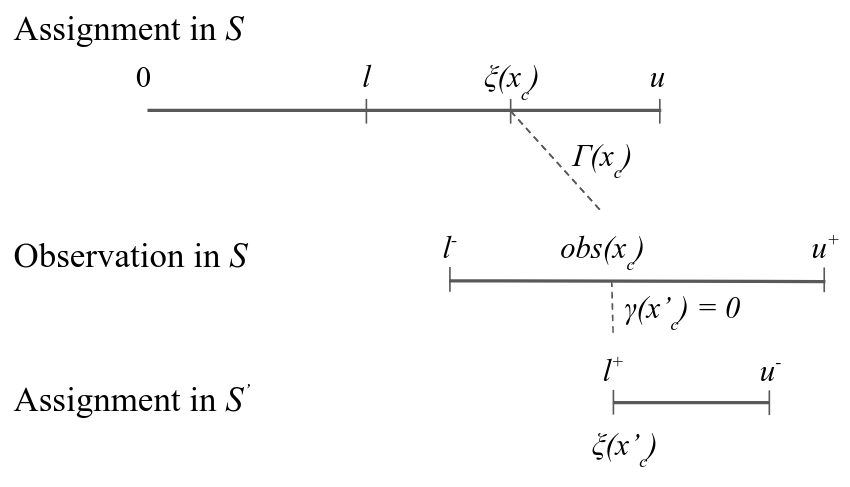
\includegraphics[width=.9\linewidth]{chapters/viz-eqn-obs-assign.png}
\caption{\label{fig:obs-assign}We visualize the relationship between realized assignments across \(S\) and \(S'\). In this example, each horizontal line is a timeline monotonically increasing from left to right. Dashed lines represent observation delays. We see how an assignment in \(S\), \assign(x\textsubscript{c})\$, realized observation delay, \(g(x_{c})\), and an observation in \(S\), \(\obs(x_{c})\), lead to an assignment in \(S'\), \assign(x'\textsubscript{c})\$.}
\end{figure}

Note that we receive \(\obs(x_{c})\) from Nature, but make the assignment \(\xi(x'_{c})\) in the
dispatchable form of \(S'\). To be clear, while \(\assign(x_{c})\) is an interval, \((\mathbb{R} \cup
\infty) \times (\mathbb{R} \cup \infty)\), \(\assign(x'_{c})\) is in \(\mathbb{R}\). For a fixed
interval, e.g. \(\obs(x_{c}) \in [t, t]\), we sometimes employ an equivalent representation,
\(\assign(x_{c}) = t\).


Additionally, we sometimes apply \(-\) and \(+\) superscripts to \(l\) and \(u\) to denote the earliest and
latest times respectively that an assignment at those bounds could be observed. For instance, the
relationship in Definition \ref{defn:vdc-obs} simplifies to,

\begin{align}
\label{eqn:obs-assign}
\label{eqn:obs-assign}
\obs(x_{c}) &= [l + \gammabar^-(x_{c}), u + \gammabar^+(x_{c})] \\
\obs(x_{c}) &= [l^-(x_{c}), u^+(x_{c})]
\end{align}

Lastly, we need a means to compare observation spaces if we are to transform variable-delay to
fixed-delay STNUs.

\begin{defn}
\textbf{Observation Space Mapping}

Let \(\mu\) be a mapping from an assignment to a situation, \(\mu : \xi \rightarrow \omega\). To say
that \(\mu(x'_{c}) \subseteq \omega_{v}(x_{c})\) means that, for any assignment of \(x'_{c}\) in \(S'\),
there is an equivalent situation in \(S\) for \(x_{c}\).
\end{defn}

For the transitions below, it is a \emph{valid observation space mapping}, if we can show that
\(\mu(x'_{c}) \subseteq \omega_{v}(x_{c})\). If so, it is guaranteed that any assignment in the
observation space of \(x'_{c}\) also has a valid assignment in the observation space of \(x_{c}\).

We now have the necessary vocabulary and notation to step through the transformations from \(S\) to
\(S'\). These lemmas were first presented in \citeprocitem{1}{[1]}.

\begin{defn}
\textbf{Variable-Delay to Fixed-Delay Transformations}

The \emph{variable-delay to fixed-delay transformations} define a set of observation space mappings,
where there are valid observation space mappings for all the contingent constraints in \(S'\) to \(S\).
\end{defn}

Thus, if there is a satisfying \(\mathcal{S}\) for the fixed-delay observation space of \(S'\), it is guaranteed to
simultaneously satisfy any situation in the variable-delay observation space, \(\Omega_{v}\), of \(S\).

\begin{lemma}
\label{lemma:emulating-fixed}
For any contingent event \(x_c \in X_c\) in \(S\), if \(\gammabar^-(x_c) = \gammabar^+(x_c)\), we emulate
\(\gammabar(x_c)\) in \(S'\) using \(\gamma(x'_c) = \gammabar^+(x_c)\).
\end{lemma}

\begin{proof}
We translate an already fixed-bounded observation delay in the form of \(\gammabar(x_{c})\) to the
equivalent fixed-delay function, \(\gamma(x'_{c})\), thus \(\omega_{f}(x'_{c}) = \omega_{v}(x_{c})\).
\end{proof}

\begin{lemma}
\label{lemma:partially-unobservable}
For any contingent event \(x_c \in X_c\), \(\gammabar^+(x_c) = \infty\), we emulate \(\gammabar(x_c)\) in
\(S'\) as \(\gamma(x'_c) = \infty\).
\end{lemma}

\begin{proof}
There are projections where we would not receive information about \(x_{c}\), therefore we have to act
as if we \emph{never} receive an observation of \(x_{c}\). Any \(\mathcal{S}\) that works when we do not
receive information about \(x_{c}\) would also work when do receive an observation if we choose to
ignore the observation.

None of our decisions depend on \(\xi(x'_{c})\), thus no observation space mapping to \(S\) is
necessary.
\end{proof}

\begin{lemma}
\label{lemma:not-enough-information}
If \(u - l \leq \gammabar^+(x_c) - \gammabar^-(x_c)\), we emulate \(\gammabar(x_c)\) in \(S'\) using
\(\gamma(x'_c) = \infty\).
\end{lemma}

\begin{proof}
We can ignore observations of \(x_{c}\) because they are not guaranteed to narrow where \(\assign(x_c)\)
was assigned in the range \([l, u]\).

Let \(\alpha\) be the range of \(\obs(x_{c})\) when \(\assign(x_{c}) \in [l, l]\). Let \(\beta\) be the
range of \(\obs(x_{c})\) when \(\assign(x_{c}) \in [u, u]\). By Equation \ref{eqn:obs-assign},

\begin{align*}
\alpha &= [l^-(x_{c}), l^+(x_{c})] \\
\beta &= [u^-(x_{c}), u^+(x_{c})]
\end{align*}

We can show that \(u^-(x_{c}) \leq l^+(x_{c})\).

\begin{align*}
u - l &\leq \gammabar^+(x_c) - \gammabar^-(x_{c}) \\
u + \gammabar^-(x_{c}) &\leq l + \gammabar^+(x_{c}) \\
u^-(x_{c}) &\leq l^+(x_{c})
\end{align*}

The lower bound of \(\beta\) is less than the upper bound of \(\alpha\), thus \(\alpha \cap \beta\). An
observation \(\obs(x_{c}) \in [u^-(x_{c}), l^+(x_{c})]\) could be the result of \(\assign(x_{c}) = [l,
l]\), \(\assign(x_{c}) = [u, u]\), or any value \(\assign(x_{c}) \in [l, u]\). Observations provide no
information about the underlying contingent constraint, therefore we ignore \(\obs(x_{c})\).

None of our decisions depend on \(\xi(x'_{c})\), thus no observation space mapping to \(S\) is
necessary.
\end{proof}

\begin{lemma}
\label{lemma:main-tightening}
If \(u - l \geq \gammabar^+(x_c) - \gammabar^-(x_c)\), we can emulate \(\gammabar(x_c)\) under minimal
information by replacing the bounds of \(x_c\) with \(x'_{c} \in [l^+(x_{c}), u^-(x_{c})]\) and letting
\(\gamma(x'_c) = 0\).
\end{lemma}

\begin{proof}
Under Lemma \ref{lemma:main-tightening}, observations \(\obs(x_{c})\) are guaranteed to narrow the range of
\assign(x\textsubscript{c})\$.

We have the same ranges for \(\alpha\) and \(\beta\) as in Lemma \ref{lemma:not-enough-information}, however
we can show that \(u^-(x_{c}) \geq l^+(x_{c})\) instead.

\begin{align*}
u - l &\geq \gammabar^+(x_c) - \gammabar^-(x_{c}) \\
u + \gammabar^-(x_{c}) &\geq l + \gammabar^+(x_{c}) \\
u^-(x_{c}) &\geq l^+(x_{c})
\end{align*}

Thus, receiving an observation is guaranteed to narrow the derived range of \(\assign(x_{c})\). The
transformation tightens the range of \(x'_{c}\) to one where there is maximum ambiguity of the
assignment of \(x_{c}\) while guaranteeing an execution strategy for any assignment of \(x_{c} \in [l,
u]\).

Based on the derivations above, it is clear that \(\mu(x'_{c})\) maps to the observation space where
there is ambiguity as to the projection of \(\assign(x_{c}) \in [l, u]\). We must also show that
\(\mu(x'_{c})\) has mappings to the extrema of \(\xi(x_{c})\). We start with the earliest
\(\assign(x'_{c})\).

$$
\assign(x'_{c}) = l^+(x_{c}) = l + \gammabar^+(x_{c})
$$

We show that that this assignment of \(\xi(x'_{c})\) can be modeled as the following observation in
\(S\).

\begin{align*}
\obs(x_{c}) &\in [l + \gammabar^-(x_{c}), l + \gammabar^+(x_{c})] \\
\obs(x_{c}) &\in [l, l] + \Gamma(x_{c})
\end{align*}

It is possible that \(\xi(x_{c}) = [l, l]\). As such, all observations in \(\obs(x_{c})\) may share the
same execution strategy because the underlying temporal constraints depend on \(\xi(x_{c})\), not
\(\obs(x'_{c})\) or \(\Gamma(x_{c})\). We may expand the range of the observation space when we map to
\(S\) with \(\mu(x'_{c})\).

\begin{align*}
\mu &: l^+(x_{c}) \rightarrow \omega_{v}(x_{c}) \\
\omega_{v}(x_{c}) &= [l + \gammabar^{-}(x_{c}), l + \gammabar^+(x_{c})]
\end{align*}

We see that \(\mu\) has a valid observation space mapping to the minimum of the range of
\(\omega_{v}(x_{c})\). We use the same argument for the maximum.

$$
\assign(x'_{c}) = u + \gammabar^-(x_{c})
$$

Observations anywhere in \([u + \gammabar^-(x_{c}), u + \gammabar^+(x_{c})]\) may share execution
strategies because, it is possible that in all cases, \(\xi(x_{c}) = [u, u]\). We may then expand the
range of the observation space when we map to \(S\).

\begin{align*}
\mu &: u^-(x_{c}) \rightarrow \omega_{v}(x_{c}) \\
\omega_{v}(x_{c}) &= [u + \gammabar^{-}(x_{c}), u + \gammabar^+(x_{c})]
\end{align*}

Thus, \(\mu(x'_{c})\) maps to the maximum of the range of \(\omega_{v}(x_{c})\). The transition creates
assignments in \(S'\) that map to the entire \(\omega_{v}(x_{c})\) in \(S\).

\end{proof}

This concludes the modifications required to transform a contingent event \(x_{c} \in X_{c}\) in \(S\)
to its equivalent \(x'_{c} \in X_{c}\) in \(S'\). What remains is to address the transformation of
requirement links, \(x_{r} \in X_{r}\), in \(S\) such that their transformed equivalents, \(x'_{r} \in
X_{r}\) in \(S'\), express the same execution semantics in \(S'\) as they did in \(S\). We will demonstrate
the correctness of the transformations after Lemma \ref{lemma:applied-execution}.

\begin{lemma}
\label{lemma:execution}
If we have contingent link \(\conedge{X}{C}{}\) with duration \([l, u]\), outgoing requirement link
\(\edge{C}{Z}{}\) with duration \([u, v]\) with an unobservable \(C\), and contingent link
\(\conedge{C}{Y}{}\) with range \([\gammabar^-(x_{c}), \gammabar^+(x_{c})]\), we can emulate the role of
the original requirement link during execution with a new link \(\edge{Y}{Z}{}\) with bounds \([u -
max(\gammabar^-(x_{c}), XY - u), v - min(\gammabar^+(x_{c}), XY - l)]\), where \(XY\) is the true
duration of \(\conedge{X}{Y}{}\).
\end{lemma}

\begin{proof}
See Figure \ref{fig:combined-figure}c for reference. From an execution perspective, \(X\) and \(Y\) are
the only events that can give us any information that we can use to reason about when to execute \(Z\)
(since \(C\) is wholly unobservable).

If we execute \(Z\) based on what we learn from \(Y\), then we use our information from \(Y\) to make
inferences about the true durations of \(\conedge{X}{C}{}\) and \(\conedge{C}{Y}{}\) based on
\(\conedge{X}{Y}{}\). We know that the lower-bound of \(\conedge{C}{Y}{}\) is at least \(XY - b\) and that
its upper-bound is at most \(XY - a\). But we also have the a priori bounds on the contingent link
that limit its range to \([\gammabar^-, \gammabar^+]\). Taken together, during execution we can infer
that the true bounds of \(\conedge{C}{Y}{}\) are \([max(\gammabar^-, XY - b), min(\gammabar^+, XY -
a)]\). Since we have bounds only on \(Z\)'s execution in relation to \(C\), we can then infer a
requirement link \(\edge{Y}{Z}{}\) with bounds \([u - max(\gammabar^-, XY - b), v - min(\gammabar^-,
XY - a)]\).

If we try to execute \(Z\) based on information we have about \(X\), we must be robust to any possible
value assigned to \(\conedge{X}{C}{}\). This means that we would be forced to draw a requirement link
\(\edge{X}{Z}{}\) with bounds \([u+b, v+a]\). But we know that \(u - max(\gammabar^-, XY - b) \leq u +
b - XY\) and \(v - min(\gammabar^-, XY - a) \geq v + a - XY\), which means that the bounds we derived
from \(Y\) are at least as expressive as the bounds that we would derive from \(X\).
\end{proof}

Since we have a local execution strategy that depends on the real value of \(XY\), we can try to apply
this strategy to the contingent link that we restricted in Lemma \ref{lemma:main-tightening}, in
order to repair the remaining requirement links.

\begin{lemma}
\label{lemma:applied-execution}
If we have an outgoing requirement link \(\edge{C}{Z}{}\) with duration \([u, v]\), where \(C\) is a
contingent event, we can emulate the role of the original requirement link by replacing its bounds
with \([u - \gammabar^-(x_{c}), v - \gammabar^+(x_{c})]\).
\end{lemma}

\begin{proof}
See Figure \ref{fig:combined-figure}d for reference. If we directly apply the transformation from
Lemma \ref{lemma:execution} and Figure \ref{fig:combined-figure}c to our original STNU, we introduce
complexity through the need to reason over \(min\) and \(max\) operations in our link bounds. However,
from Lemma \ref{lemma:main-tightening}, we know that in a controllability evaluation context, it is
acceptable for us to simplify the \(\conedge{X}{Y}{}\) link to a stricter range of \([a + \gammabar^+,
b + \gammabar^-]\), instead of \([a + \gammabar^-, b + \gammabar^+]\). This means that for the purpose
of evaluating controllability, we can assume \(a + \gammabar^+ \leq XY \leq b + \gammabar^-\). When we
evaluate the requirement link \(\edge{Y}{Z}{}\), we see \(max(\gammabar^-, XY - b) = \gammabar^-\) and
\(min(\gammabar^+, XY - a) = \gammabar^+\). This gives us bounds of \([u - \gammabar^-, v -
\gammabar^+]\) for the \(\edge{Y}{Z}{}\) requirement link as seen in Figure \ref{fig:combined-figure}d.
\end{proof}

Lemma \ref{lemma:applied-execution} handles outgoing requirement edges connected to contingent
events. In addition, we must handle incoming edges.

\begin{corollary}
\label{corollary:reversed}
If we have an incoming requirement link \(\edge{Z}{C}{}\) with duration \([u, v]\), where \(C\) is a
contingent event, we can replace the bounds of the original requirement link with \([u +
\gammabar^+(x_{c}), v + \gammabar^-(x_{c})]\).
\end{corollary}

\begin{proof}
A requirement link \(\edge{Z}{C}{}\) with bounds \([u, v]\) can be immediately rewritten as its reverse
\(\edge{C}{Z}{}\) with bounds \([-v, -u]\). After reversing the edge, we can apply Lemma
\ref{lemma:applied-execution} to get \(\edge{Y}{Z}{}\) with bounds \([-v - \gammabar^-, -u -
\gammabar^+]\), which we can reverse again to get \(\edge{Z}{Y}{}\) with bounds \([u + \gammabar^+, v +
\gammabar^-]\).
\end{proof}

After applying Lemma \ref{lemma:main-tightening}, despite the limited expected range of assignments in
\(x'_{c}\) in \(S'\) compared to \(x_{c}\) in \(S\), we can show that Lemma \ref{lemma:applied-execution}
guarantees a satisfying schedule for any \(\obs(x_{c}) \in [l^-(x_{c}), u^+(x_{c})]\) using an
\(\mathcal{S}\) that employs \emph{buffering} and \emph{imagining} contingent events.

\begin{defn}
\textbf{Buffering}

\emph{Buffering} a contingent event \(x_{c}\) is an execution strategy where, if \(x_{c}\) is observed
earlier than the lower bound of the observation space \(\obs(x_{c}) < \omega_{f}^-(x'_{c})\), we
assign \(\xi(x'_{c})\) to the lower bound of the observation space, \(\xi(x'_{c}) =
\omega_{f}^-(x'_{c})\).
\end{defn}

\begin{defn}
\textbf{Imagining}

\emph{Imagining} a contingent event \(x_{c}\) is an execution strategy where, if \(x_{c}\) is observed later
than the upper bound of the observation space, \(\obs(x_{c}) > \omega_{f}^+(x'_{c})\), we assign
\(\xi(x'_{c})\) to the upper bound of the observation space, \(\xi(x'_{c}) = \omega_{f}^+(x'_{c})\).
\end{defn}

\begin{lemma}
If \(S'\) is fixed-delay controllable after applying Lemmas \ref{lemma:main-tightening}, \ref{lemma:execution},
and \ref{lemma:applied-execution} to contingent event \(Y\) with following requirement event \(Z\), there is a
valid \(\mathcal{S}\) for any observation in the observation space of \(S\), \(\omega_{v}(Y) = [a^-(Y),
b^+(Y)]\).
\end{lemma}

\begin{proof}
We first note the observation space of \(S'\) is a subinterval of the original observation space of
\(S\), \(\omega_{f}(Y') \subset \omega_{v}(Y)\), and there are two distinct ranges of observations that
are not in \(\omega_{f}(Y')\).

\begin{align*}
\omega_{f}(Y') &= [a + \gammabar^+(Y), b + \gammabar^-(Y)];~\omega_{v}(Y) = [a + \gammabar^-(Y), b + \gammabar^+(Y)] \\
\omega_{f}(Y') &\not\supset [a + \gammabar^-(Y), a + \gammabar^+(Y))~~(\textit{"Early" observations}) \\
\omega_{f}(Y') &\not\supset (b + \gammabar^+(Y), b + \gammabar^+(Y)]~~(\textit{"Late" observations})
\end{align*}

We address the early observations first. The range of early assignments of \(\xi(Y)\) in \(S\) that we
care about are the ones that could produce an observation \(\obs(Y) \leq a + \gammabar^+(Y)\), which
is \(\xi(Y) = [a, a + (\gammabar^+(Y) - \gammabar^-(Y))]\). We rewrite the range of early assignments
as \(\xi(Y) = a + (\gammabar^+(Y) - \gammabar^-(Y)) - \epsilon\), where \(0 \leq \epsilon \leq
(\gammabar^+(Y) - \gammabar^-(Y))\). By the semantics of \(S\), the range of assignments of \(\xi(Z)\) is
then,

\begin{align*}
\xi(Z) &= [a + (\gammabar^+(Y) - \gammabar^-(Y)) - \epsilon, a + (\gammabar^+(Y) - \gammabar^-(Y)) - \epsilon] + [u, v] \\
\xi(Z) &= [a + u + (\gammabar^+(Y) - \gammabar^-(Y)) - \epsilon, a + v + (\gammabar^+(Y) - \gammabar^-(Y)) - \epsilon]
\end{align*}

The earliest assignment of \(Y'\) in \(S'\) is \(\xi(Y') = a + \gammabar^+(Y)\). By the semantics of \(S'\),
the range of assignments of \(\xi(Z')\) is then,

\begin{align*}
\xi(Z') &= [a + \gammabar^+(Y), a + \gammabar^+(Y)] + [u - \gammabar^-(Y), v - \gammabar^+(Y)] \\
\xi(Z') &= [a + u + (\gammabar^+(Y) - \gammabar^-(Y)), a + v]
\end{align*}

We see that \(\xi(Z') \subseteq \xi(Z)\) for any \(\epsilon\), meaning the execution strategy when
\(\xi(Y') = a + \gammabar^+(Y)\) results in a valid assignment of \(\xi(Z)\) for all early observations
of \(\xi(Y)\). We are safe to buffer early observations to \(\xi(Y') = a + \gammabar^+(Y)\).

We use the same argument for imagining late observations. The range of late assignments of \(\xi(Y)\)
in \(S\) that we care about are the ones that could produce an observation \(\obs(Y) \geq b +
\gammabar^-(Y)\), which is \(\xi(Y) = b - (\gammabar^+(Y) - \gammabar^-(Y)) + \epsilon\). By the
semantics of \(S\), the range of assignments of \(\xi(Z)\) is then,

\begin{align*}
\xi(Z) &= [b - (\gammabar^+(Y) - \gammabar^-(Y)) + \epsilon, b - (\gammabar^+(Y) - \gammabar^-(Y)) + \epsilon] + [u, v] \\
\xi(Z) &= [b + u - (\gammabar^+(Y) - \gammabar^-(Y)) + \epsilon, b + v - (\gammabar^+(Y) - \gammabar^-(Y)) + \epsilon]
\end{align*}

The last assignment of \(Y'\) in \(S'\) is \(\xi(Y') = b + \gammabar^-(Y)\). By the semantics of \(S'\),
the range of assignments of \(\xi(Z')\) is then,

\begin{align*}
\xi(Z') &= [b + \gammabar^-(Y), b + \gammabar^+(Y)] + [u - \gammabar^-(Y), v - \gammabar^+(Y)] \\
\xi(Z') &= [b + u, b + v - (\gammabar^+(Y) - \gammabar^-(Y))]
\end{align*}

We see that \(\xi(Z') \subseteq \xi(Z)\) for any \(\epsilon\), meaning the execution strategy when
\(\xi(Y') = b + \gammabar^-(Y)\) results in a valid assignment of \(\xi(Z)\) for all late observations
of \(\xi(Y)\). In practice, there is no reason to wait until after \(\obs(Y) = b + \gammabar^-(Y)\) to
receive a late observation. As soon as we see the clock has reached \(b + \gammabar^-(Y)\), we are
safe to imagine that \(\obs(Y)\) has been received.
\end{proof}

We can examine a concrete example of Lemmas \ref{lemma:main-tightening}, \ref{lemma:execution}, and
\ref{lemma:applied-execution} to show equivalence in the transformation from Figure
\ref{fig:combined-figure}a to \ref{fig:combined-figure}d. We start by building an example of
\ref{fig:combined-figure}a. Let \(\conedge{X}{C}{[2, 5]}\) with \(\gammabar(C) \in [1, 2]\) and
\(\edge{C}{Z}{[11, 20]}\). If we learn of event \(C\) at time 4, then one possibility is that the
realized duration of \(C\) could have been 2 with an observation delay of 2. In this case, event \(Z\)
must be executed in \([13, 22]\). However, if the realized duration of \(C\) were 3 with an observation
delay of 1, then \(Z\) would fall in \([14, 23]\). Given we cannot distinguish between the
possibilities, we take the intersection of the intervals, yielding \(Z \in [14, 22]\). Likewise, if we
learn of \(C\) at time 6, then \(C\) could have been realized at time 5 with an observation delay of 1
or it could have been realized at time 4 with an observation delay of 2. In the first case, \(Z\) must
then fall in \([16, 25]\), while in the second, \(Z\) would fall in \([15, 24]\). The intersection yields
\([16, 24]\).

By the semantics represented in Figure \ref{fig:combined-figure}d, we can build an equivalent
network with \(\gamma(Y) = 0\) by setting \(\conedge{X}{Y}{[4, 6]}\) and \(\edge{Y}{Z}{[10, 18]}\). If \(Y\)
is observed at time 4, \(Z\) must be executed in \([14, 22]\). If \(Y\) is observed at time 6, \(Z\) then
must be executed in \([16, 24]\). The execution semantics for both cases match the equivalent networks
from \ref{fig:combined-figure}a described above.

\section{Dynamic Scheduling through Real-Time Execution Decisions}
\label{sec:org978a146}
\label{sec:dynamic-scheduling}

An STNU, \(S\), that exhibits dynamic controllability can be \emph{scheduled} dynamically (or \emph{online}). At
a high-level, dynamic scheduling is the process of mapping the history of event assignments to the
execution time of future free events. We follow the scheduling work by Hunsberger
\citeprocitem{36}{[36]}, \citeprocitem{38}{[38]}, which describes an \(O(N^{3})\) procedure, FAST-EX, for
dynamic scheduling of STNUs. At its core is the notion of \emph{Real-Time Execution Decisions} (RTEDs),
which map a timepoint to a set of requirement events to be executed and are generated based on
\emph{partial schedules} of STNUs being executed. \texttt{WAIT} decisions may also be produced, reflecting the
need to wait for the assignment of a contingent event before continuing. RTED-based scheduling
applies a dynamic programming paradigm by first creating a dispatchable form of temporal constraints
offline, updating the dispatchable form as the partial schedule is updated online, and querying the
dispatchable form online to quickly find the next free event to schedule \citeprocitem{39}{[39]}.

\begin{defn}
\textbf{Real-Time Execution Decisions} \citeprocitem{39}{[39]}

A \emph{Real-Time Execution Decision} is a two-tuple \(\langle t, \chi \rangle\), where:
\begin{itemize}
\item \(t\) is a time with domain \(\mathbb{R}\),
\item \(\chi\) is a set of \(x_{r} \in X_{r}\) to be executed at time \(t\)
\end{itemize}
\end{defn}

\begin{defn}
\textbf{Partial Schedule}

A \emph{Partial Schedule} for an STNU is a mapping \(\xi ~:~ t \rightarrow \mathbb{R}\), where \(t\) is a
proper subset of timepoints in \(X\) with domain \(\mathbb{R}\).
\end{defn}

A partial schedule is the set of assignments \emph{so far} during execution. They can be represented by
\(\xi_{t} = \{ (A, \xi(A) \}\) notation, meaning that by some time \(t\), event \(A\) has been scheduled
at time \(\xi(A)\). By definition, all STNU executions begin with a partial schedule \(\xi_{0} =
\emptyset\), meaning no timepoints have been assigned at time \(0\). As timepoints are executed, the
partial schedule grows. For example, if event \(A\) is assigned to \(1\) and \(B\) to \(2\), then at time
\$2, \(\xi_{2} = \{ (A, 1), (B, 2) \}\).

The dispatchable form employed by FAST-EX is the \emph{AllMax} distance graph, which is produced by the
Morris \(O(N^{4})\) DC-checking procedure \citeprocitem{27}{[27]}.

\begin{defn}
\textbf{AllMax Distance Graph} \citeprocitem{26}{[26]}

The \emph{AllMax} distance graph is a distance graph exclusively consisting of unlabeled and upper-case
edges.
\end{defn}

The key idea of FAST-EX is maintaining accurate distances from a zero point, \(Z\), of the graph to
all events. At the outset of execution, all events from \(S\) are present as nodes in \emph{AllMax}. As
contingent events are observed, \emph{AllMax} performs update steps using Dijkstra Single Source/Sink
Shortest Path (SSSP) to maintain distances to unexecuted events, while also removing executed
events. We include pseudo-code of the update step in Figure \ref{alg:fast-ex-update}.

\begin{algorithm}
\SetAlgoLined
\SetKwFunction{Return}{return}
\SetKwInput{Input}{Input}
\SetKwInput{Output}{Output}
\SetKwInput{Algorithm}{\textsc{FAST-EX Update}}
\SetKwInput{Initialize}{Initialization}
\SetKwIF{If}{ElseIf}{Else}{if}{then}{else if}{else}{endif}
\Indm
\Input{Time $t$; Set of newly executed events $\texttt{Exec} \subseteq X_{e} \cup X_{r}$; AllMax Graph $G$; Distance matrix $D$, where $D(A, B)$ is the distance from $A$ to $B$}
\Output{Updated $D$}
\Indp
\Algorithm{}
\Indp
\For{each continent event $C \in \texttt{Exec}$} {
    Remove each upper-case edge, $\edge{Y}{A}{C:-w}$, labled by $C$\;
    Replace each edge from $Y$ to $Z$ with the strongest replacement edge\;
}
\For{each event $E \in \texttt{Exec}$} {
    Add lower-bound edge $\edge{E}{Z}{-t}$\;
}
For each event $X$, update $D(X, Z)$ using Dijkstra Single-Sink Shortest Paths\;
\For{each event $E \in \texttt{Exec}$} {
    Add upper-bound edge $\edge{Z}{E}{t}$\;
}
For each event $X$, update $D(Z, X)$ using Dijkstra Single-Source Shortest Paths\;
\caption{Algorithm for updating distances for all events in relation to $Z$ upon the execution of an event. Adapated from \citeprocitem{3}{[3]}, Fig. 19.}
\label{alg:fast-ex-update}
\end{algorithm}

Given an accurate distance matrix, we find the next RTED as follows. Let \(U_{x}\) be the set of
unexecuted free timepoints. If \(U_{x}\) is empty, then the RTED is to \texttt{WAIT}. Otherwise, we find the
lower bound of the earliest executable time point and the set of executable events associated with
it.

\begin{align*}
t &= \min\{-D(X, Z)~|~X \in U_{x}\} \\
\chi &= \{X \in U_{x}~|~-D(X, Z) = t\}
\end{align*}

We cannot execute events in the past. Let \(\texttt{now}\) be the current time, i.e. the last timepoint
captured in \(\xi\). It is possible that \(t \leq \texttt{now}\), in which case we must reassign \(t\) to
guarantee that \(t > \texttt{now}\). To do so, we update \(t\) as follows, where \(t_{U}\) is earliest
\emph{upper} bound of the executable timepoints,

\begin{align*}
t_{U} &= \min\{D(Z, X)~|~X \in U_{x}\} \\
t &= \cfrac{\texttt{now} + t_{U}}{2}
\end{align*}

So long as \(t_{U} > \texttt{now}\), we know that the reassignment of \(t\) ensures \(t > \texttt{now}\).

\chapter{Dynamic Scheduling with Delayed Event Monitoring}
\label{sec:org50bc965}
\label{ch:delay-scheduling}

\begin{figure}[htbp]
\centering
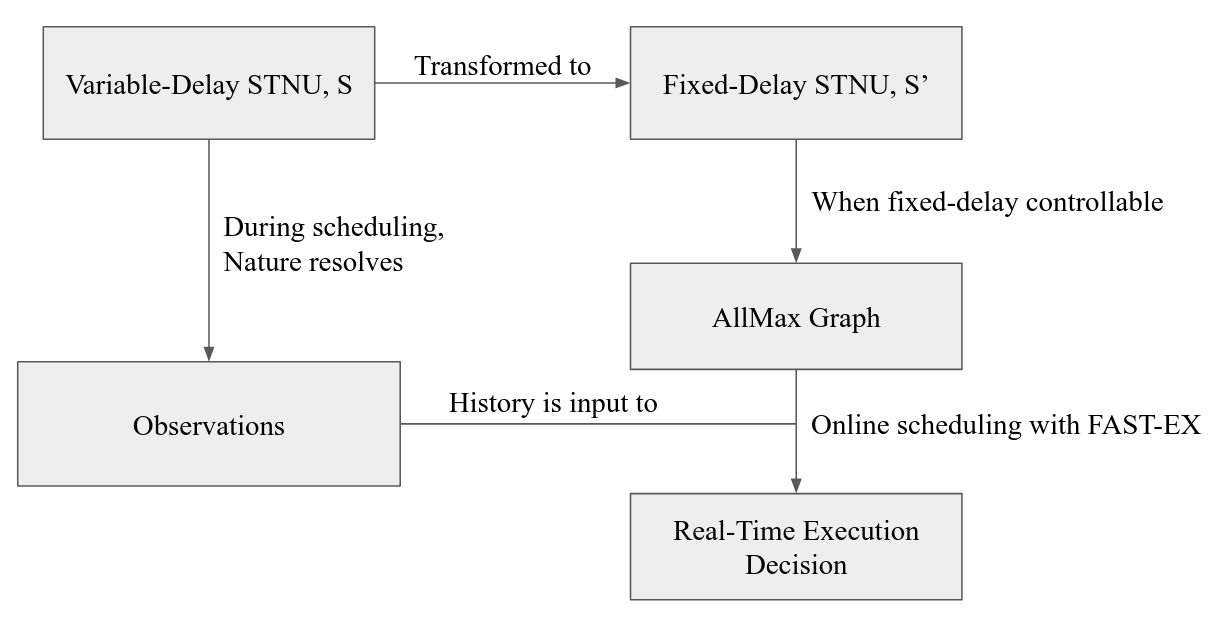
\includegraphics[width=2.5in]{chapters/flow-chart.png}
\caption{\label{fig:flow-chart}From a variable-delay STNU to scheduling decision}
\end{figure}

This section represents the start of contributions from this paper. Our aim is to describe \emph{delay
scheduling}, an RTED-based strategy for dispatching free events in the case where there is
set-bounded observation delay for contingent events. As will be shown, delay scheduling is an
extension to dynamic scheduling using the execution strategy as outlined in the variable-delay
controllability checking procedure.

We must address three gaps: first, we reconcile

At the conclusion of this Section, we extend our approach to scheduling variable-delay STNUs by
introducing an optional procedure that addresses a shortcoming in the semantics of scheduling a
variable-delay STNU. The shortcoming takes the form of potentially unnecessary wait times that are
added after receiving contingent event assignments, extending the makespan of procedures. We present
a generate-and-test algorithm to partially mitigate said shortcomings.

Bhargava et al. \citeprocitem{1}{[1]} addressed this ambiguity in contingent event assignment by
first transforming the VDC STNU into a controllability-equivalent fixed-delay STNU. With fixed
observation delay, we \emph{do} have the guarantee that we learn the exact assignment of contingent
events (so long as the observation delay is not infinite). Thus, scheduling a fixed-delay STNU only
differs from scheduling a vanilla STNU in that we must subtract a fixed observation delay when we
make contingent event assignments. Otherwise, the dispatchable form is the same as in the case of a
vanilla STNU, and we can choose any STNU scheduling algorithm to generate execution decisions.

The flow from variable-delay STNU to fixed-delay STNU to dispatchable form may appear sufficient to
enable scheduling of variable-delay STNUs, but we must contend with a novel issue: the execution
spaces of the original variable-delay STNU and its transformed fixed-delay equivalent are
mismatched. Nature is obliged to respect the uncertainties of the original variable-delay STNU. As
will be shown later, the fixed-delay equivalent reduces the execution space to make the
controllability check tractable. As such, we may receive observations outside the range of the
contingent links in the fixed-delay STNU, which we must reconcile with the dispatchable form. See
Figure \ref{fig:flow-chart} for an overview of the information flow in scheduling a variable-delay STNU.

\section{Scheduling with Variable-Observation Delay}
\label{sec:orgafc35ca}

To solidify the process of scheduling a variable-delay STNU, consider the following analogy.

\begin{quote}
Alex wants to go hiking in the woods. The area is unfamiliar to them, so they ask their friend, Sam,
who hiked these trails a long time ago, to give them directions to traverse from the trailhead to a
particularly spectacular overlook. Sam has a working idea of the trail map, but their memory is
imperfect. Regardless, they guarantee Alex that their directions will lead Alex to the overlook even
if the woods have changed over the years. Sam writes down directions like ``turn left after 500
meters at the giant oak tree'' and ``turn right after 100 meters when you see the brook.'' Alex knows
that Nature will not necessarily obey Sam's directions. They may observe a giant oak tree earlier
than expected, so they must then wait to take the next trail going left. Or the brook may have dried
up, so they imagine they saw one near where Sam thought it would be and take the next right. While
hiking, Alex is charged with reconciling Sam's directions with their own observations. Even though
they may identify the landmarks in Sam's directions earlier or later than expected, their actions
will need to follow Sam's instructions to maintain the guarantee of reaching the overlook.
\end{quote}

In our analogy, \(S\) models the current state of the hiking trails and the full range of projections,
while \(S'\) is Sam's working memory of them. Sam's directions are the execution strategy described by
the AllMax graph we get by checking the fixed-delay controllability of \(S'\). Observations of Nature
obey \(S\). Alex is charged with reconciling their observations from \(S\) with Sam's hiking directions
from \(S'\). The analogy ends here, though, as the math and logic of temporal reasoning do not neatly
translate into hiking. Luckily, we have more information than Alex. Unlike human memory, which is
untrustworthy and irrational, the fixed-delay STNU, \(S'\), is created by a set of Lemmas with
deterministic outcomes. As such, we have the means to interpret how observations in \(S\) \emph{would
appear} in \(S'\), which will be critical in adapting our fixed-delay execution strategy in response
to variable observation delay.

Our key challenge for scheduling an STNU with variable observation delay is reconciling observations
from \(S\) with the dispatchable form from \(S'\).

\section{Recording Contingent Event Assignments}
\label{sec:orge3f6713}
\label{sec:recording-vdc-ctg}

During execution, we observe the outcome of contingent events \(\obs(x_{c})\) in \(S\), but we make
assignments in the dispatchable form of \(\assign(x'_{c})\) in \(S'\). Despite being equivalent with
respect to controllability, the bounds of contingent links \(x_{c}\) in \(S\) and \(x'_{c}\) in \(S'\) are
not equivalent.

We need a modified procedure for contingent event assignments that wraps FAST-EX. No
modifications to FAST-EX are necessary to schedule fixed-delay STNUs because checking FDC includes
the procedure of creating the same AllMax graph that FAST-EX requires.

We now present our strategy for recording observations during execution as derived from the
transformations outlined in Section \ref{sec:vdc}.

\begin{lemma}
\label{lemma:information-fixes-bounds}
For any contingent event, $x_{c} \in S$ or $x'_{c} \in S'$, observing $x_{c}$ at time $t \in [l^-(x_{c}), u^+(x_{c})]$ fixes the observation to $\obs(x_{c}) = [t, t] = t$.
\end{lemma}

\begin{proof}

Prior to execution, observations are defined as set-bounded intervals from the earliest possible
observation at \(l^-(x_{c})\) to the last possible observation at \(u^+(x_{c})\). Receiving an
observation \(\obs(x_{c}) = t\) during execution eliminates all members of the pre-execution interval
except \(t\).
\end{proof}

\begin{lemma}
\label{lemma:ignore-inf-delay}
For any contingent event $x'_{c} \in X_{c}$ in fixed-delay controllable $S'$, if $\gamma(x'_{c}) = \infty$, we mark the event executed but do not assign \assign(x'_{c})$ in the dispatchable form of $S'$.
\end{lemma}

\begin{proof}
If we are scheduling a fixed-delay STNU, \(S'\), that is already known to be fixed-delay controllable,
an execution strategy must exist that is independent of the assignment of \(\assign(x'_{c})\) when
\(\gamma(x'_{c}) = 0\). We are not required to record \(\assign(x'_{c})\) when \(\gamma(x'_{c}) = \infty\)
to guarantee controllability and may safely ignore it.

We mark the event executed to prevent it from appearing in future RTEDs.

\end{proof}

Lemma \ref{lemma:ignore-inf-delay} may be applicable to any contingent events, \(x'_{c} \in X_{c}\) in \(S'\)
that were transformed from the variable-delay form \(S\) using Lemmas \ref{lemma:emulating-fixed},
\ref{lemma:partially-unobservable}, or \ref{lemma:not-enough-information}.

\begin{lemma}
\label{lemma:subtract-gamma}
For any contingent event $x'_{c} \in X_{c}$ in fixed-delay controllable $S'$, if $\gamma(x'_{c}) \in \mathbb{R}$, we assign $\assign(x'_{c}) = \obs(x_{c}) - \gamma(x'_{c})$ in the dispatchable form of $S'$.
\end{lemma}

\begin{proof}
The central challenge of checking fixed-delay controllability is determining that an execution
strategy exists that allows an agent to wait an additional \(\gamma(x'_{c})\) time units after a
contingent event has been assigned to learn its outcome. Importantly, the \(\gamma\) function is not
used to modify the edges of the labeled distance graph, which are derived from the constraints \(r
\in R_{e} \cup R_{c}\) in \(S'\).

As \(\gamma(x'_{c})\) resolves to a known and finite value, we can derive the true value of
\assign(x'\textsubscript{c})\$ to be assigned in the labeled distance graph. Contingent event assignments, \assign(x'\textsubscript{c})\$,
are recorded in the labeled distance graph as follows, where \(\obs(x_{c})\) is the resolved observation,

\begin{align}\assign(x'_c) = \obs(x_c) - \gamma(x'_c) \label{eqn:fixed-recording}
\end{align}
\end{proof}

Next, in comparing the bounds of \(x_{c}\) and \(x'_{c}\) when \(u - l \geq \gammabar^+(x_c) -
\gammabar^-(x_c)\), \(x'_{c} \in [l^+(x_{c}), u^-(x_{c})]\) (Lemma \ref{lemma:main-tightening}) there are
three regimes of observations of \(\obs(x_{c})\) we must consider:

\begin{enumerate}
\item \(\obs(x_{c}) \in [l^-(x_{c}), l^+(x_{c}))\), ie. strictly earlier than the range of \(\assign(x'_{c})\),
\item \(\obs(x_{c}) \in [l^+(x_{c}), u^-(x_{c})]\), ie. the range equivalent to \(x'_{c}\), and
\item \(\obs(x_{c}) \in(u^-(x_{c}), u^+(x_{c})]\), ie. strictly later than the range of \(\assign(x'_{c})\).
\end{enumerate}

Nature decides in which regime we receive \(\obs(x_{c})\). We are faced with the unique challenge of
deciding how to act when Nature selects an \(\obs(x_{c})\) that fails to follow the constraints of
\(S'\), eg. \(\obs(x_{c}) < l^+(x_{c}) \lor \obs(x_{c}) > u^-(x_{c})\), which would lead to an
assignment, \(\assign(x'_{c})\), in the first or third regimes above. In plainer words, the contingent
links of \(S\) and \(S'\) do not have the same constraints. We make assignments in \(S'\), but we receive
observations from \(S\). We need to decide how to act when we observe a contingent event earlier or
later than we expect according to \(S'\), because if we blindly assigned \(\assign(x'_{c})\) outside its
constraints from \(S'\), we lose the guarantee of controllability. Our only choice is to find a
strategy to assign \(x'_{c}\) that respects the constraints of \(S'\), despite observing \(x_{c}\) earlier
or later than expected. We do so by reasoning over the possible \emph{range} of assignments,
\(\assign(x_{c})\), that could have led to a particular observation, \(\obs(x_{c})\). What we find is
that, due to the uncertainty in observation delay, we are allowed to \emph{modify} our assignment of
\(\assign(x'_{c})\) to ensure it respects \(S'\). We present two modification strategies for addressing
the first and third cases, which we call \emph{buffering} and \emph{imagining} respectively.

We first address the case where \(\obs(x_{c}) < l^+(x_{c})\).

\begin{lemma}
\label{lemma:buffering}
If a contingent event, $x_{c} \in X_{c}$, is observed earlier than the bounds of $x'_{c}$ in $S'$ for a fixed-delay controllable $S'$, $\obs(x_{c}) < l^+(x_{c})$, we perform a \textit{buffering} operation by letting $\assign(x'_{c}) = l^+(x_{c})$ in $S'$.
\end{lemma}

\begin{proof}

\begin{figure}[htbp]
\centering
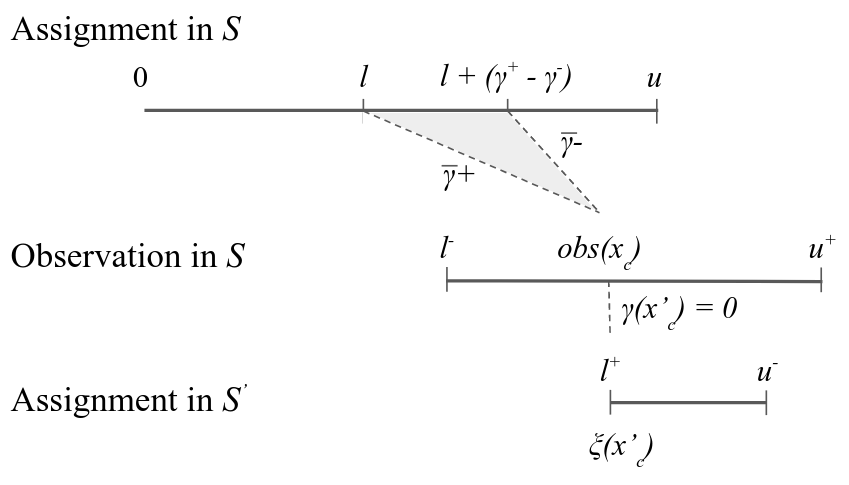
\includegraphics[width=.9\linewidth]{chapters/viz-l-plus.png}
\caption{\label{fig:observations}Here, we show how the combination of \(\assign(x_{c})\) and \(\gammabar(x_{c})\) lead to an assignment of \(\assign(x'_{c})\) in \(S'\). We see the range \(\alpha \in [l, l + \gammabar^+(x_{c}) - \gammabar^-(x_{c})\) representing the earliest and latest assignments of \assign(x\textsubscript{c})\$ that could result in \(\obs(x_{c}) \in \assign(x'_{c}) \in [l^+(x_{c})\), l\^{}+(x\textsubscript{c})]\$. The grey region represents the range of possible observation delays, \(\gammabar(x_{c})\), supporting \(\assign(x'_{c}) \in [l^+(x_{c}), l^+(x_{c})]\).}
\end{figure}

To demonstrate why buffering is sound, we compare the bounds of \(x_{c}\) in \(S\) and \(x'_{c}\) in \(S'\)
to show that our execution strategy for \(\assign(x'_{c})\) is applicable to any \(\assign(x_{c}) \in
[l, l^+(x_{c})]\).

We know that \(S'\) is fixed-delay controllable when \(\assign(x'_{c}) \in [l^+(x_{c}), u^-(x_{c})]\).
Consider an observation at the lower bound of \$\assign(x'\textsubscript{c}), \(\obs(x_{c}) = l^+(x_{c})\). We can
discern the range of possible assignments of \(x_{c}\) in \(S\) (Using Lemma
\ref{lemma:information-fixes-bounds} to rewrite \(o(x_{c}) = l^+(x_{c})\) as \(o(x_{c}) = [l^+(x_{c}),
l^+(x_{c})]\)).

\begin{align*}
\obs(x_{c}) &= \assign(x_{c}) + \gammabar(x_{c}) \\
\assign(x_{c}) &= \obs(x_{c}) - \gammabar(x_{c}) \\
\assign(x_{c}) &= [l^+(x_{c}), l^+(x_{c})] - [\gammabar^-(x_{c}), \gammabar^+(x_{c})] \\
\assign(x_{c}) &= [l, l + (\gammabar^+(x_{c}) - \gammabar^-(x_{c}))]
\end{align*}

Let \(\alpha = [l, l + (\gammabar^+(x_{c}) - \gammabar^-(x_{c}))]\) for this Lemma.

Given \(S'\) is fixed-delay controllable, there must exist an execution strategy when \(\assign(x'_{c})
= l^+(x_{c})\), which entails the same execution strategy applies for any assignment of
\(\assign(x_{c}) \in \alpha\). Thus, during execution, if we can show that \(\assign(x_{c}) \subseteq
\alpha\), we can safely act as if \(\assign(x'_{c}) = l^+(x_{c})\).

Now, let \(\obs(x_{c}) = l^+(x_{c}) - \epsilon\) for some small, positive \(\epsilon\). Accordingly, it
is the case that \(\assign(x_{c})\) must fall in the range,

\begin{align*}
\assign(x_{c}) &= [(l^+(x_{c}) - \epsilon) - [\gammabar^-(x_{c}), \gammabar^+(x_{c})] \\
\assign(x_c) &= [l^+(x_{c}) - \epsilon, l^+(x_{c}) - \epsilon] - [\gammabar^-(x_{c}), \gammabar^+(x_{c})] \\
\assign(x_c) &= [l - \epsilon, l + (\gammabar^+(x_{c}) - \gammabar^-(x_{c})) - \epsilon]
\end{align*}

Of course, \(\assign(x_{c})\) must respect the original bounds of \(x_{c}\), \(x_{c} \in [l, u]\).

\begin{align*}
\assign(x_c) &= [l - \epsilon, l + \gammabar^+(x_{c}) - \gammabar^-(x_{c}) - \epsilon] \cap [l, u]
\assign(x_c) &= [l, l + (\gammabar^+(x_{c}) - \gammabar^-(x_{c})) - \epsilon]
\end{align*}

Let \(\beta = [l, l + (\gammabar^+(x_{c}) - \gammabar^-(x_{c})) - \epsilon]\) for this Lemma. See
Figure \ref{fig:observations} for a visual representation of how an observation \(\obs(x_{c})\) is
interpreted as an assignment \assign(x'\textsubscript{c})\$ during scheduling.

We see that \(\beta \subset \alpha\). Thus, if we receive an observation \(\obs(x_{c})\) earlier than
\(l^+(x_{c})\), we may safely buffer by applying the execution strategy from an assignment of
\(\obs(x_{c}) = \assign(x'_{c}) = l^+(x_{c})\).
\end{proof}

Next,we address the case where \(\obs(x_{c}) > u^-(x_{c})\).

\begin{lemma}
\label{lemma:imagining}
If a contingent event, $x_{c} \in X_{c}$, will be observed after the bounds of $x'_{c}$, $\obs(x_{c}) > u^-(x_{c})$, we \textit{imagine} we have received it by assigning $\assign(x'_{c}) = u^-(x_{c})$ in $S'$.
\end{lemma}

\begin{proof}
We apply the same argument to \emph{imagining} late events. We now consider an observation at the upper
bounds of \(x'_{c}\), \(\obs(x_{c}) = \assign(x'_{c}) = u^-(x_{c})\). We then have a new \(\alpha\)
representing the range of the earliest and latest assignments to \(\assign(x_{c})\),

\begin{align*}
\alpha &= u^-(x_{c}) - g(x_{c}) \\
       &= [u^-(x_{c}), u^-(x_{c})] - [\gammabar^-(x_{c}), \gammabar^+(x_{c})] \\
\alpha &= [u - (\gammabar^+(x_{c}) - \gammabar^-(x_{c})), u]
\end{align*}

Once again, if \(S'\) is fixed-delay controllable, there must exist an execution strategy for
\(\assign(x'_{c}) = u^-(x_{c})\). It follows that we can apply this execution strategy when
\(\assign(x_{c}) \in \alpha\).

If we receive a late observation, \(\obs(x_{c}) = u^-(x_{c}) + \epsilon\), we find that
\(\assign(x_{c})\) must fall in the range of a new \(\beta\), where

\begin{align*}
\beta &= \left[ (u^-(x_{c}) + \epsilon) - g(x_{c}) \right] \cap [l, u] \\
      &= \left[ [u^-(x_{c}) + \epsilon, u^-(x_{c}) + \epsilon] - [\gammabar^-(x_{c}), \gammabar^+(x_{c})] \right] \cap [l, u] \\
      &= [u - (\gammabar^+(x_{c}) - \gammabar^-(x_{c})) + \epsilon, u + \epsilon] \cap [l, u] \\
\beta &= [u - (\gammabar^+(x_{c}) - \gammabar^-(x_{c})) + \epsilon, u]
\end{align*}

We find that \(\beta \subset \alpha\) again and can safely imagine that we received \(\obs(x_{c}) =
u^-(x_{c})\). Of course, we need not wait to receive a late observation of \(x_{c}\) only to assign it
to a time in the past. During execution, if we have not received \(\obs(x_{c})\) by \(u^-(x_{c})\), we
imagine an observation arrived at \(\obs(x_{c}) = u^-(x_{c})\) and thus assign \(\assign(x'_{c}) =
u^-(x_{c})\). We then ignore the real observation of \(x_{c}\) that we receive later.
\end{proof}

We have addressed the key issue of reconciling observations from \(S\) with the dispatchable form from
\(S'\). We now present a dispatcher and wrapper algorithms on top of FAST-EX that combine to add
robustness for variable observation delay.

\section{Modified FAST-EX for Variable Observation Delay}
\label{sec:orgc1c38eb}

We present an overview of the scheduling and dispatching algorithms below with explanations following.

While we made a careful distinction between \(x_{c}\) and \(x'_{c}\) in our discussion of scheduling, in
our implementation it was important to be able to easily replace one with another when looking up
values in hash-tables and lists. For instance, to implement Equation \ref{eqn:fixed-recording}, we receive
\(x_{c}\) but key the fixed-delay function on \(x'_{c}\). Rather than adding an additional translation
layer, we give each temporal event in \(S\) a unique name, all of which get copied to their equivalent
events in \(S'\). Hash-tables are keyed on event names, vastly simplifying lookups in the AllMax
graph, delay function, and elsewhere.

Let \(x\) be a temporal event, \(x \forall x \in X_{c} \cup X_{e}\).

\begin{algorithm}[H]
\SetAlgoLined
\SetKwFunction{Return}{return}
\SetKwInput{Input}{Input}
\SetKwInput{Output}{Output}
\SetKwInput{Algorithm}{\textsc{VDC-FAST-EX-Update}}
\SetKwInput{Initialize}{Initialization}
\SetKwIF{If}{ElseIf}{Else}{if}{then}{else if}{else}{endif}
\Indm
\Input{AllMax Graph $G$; fixed-delay function $\gamma(x'_{c})$; Observation $\obs(x_{c})$}
\Output{Updated AllMax Graph $G$}
\Initialize{}
\Indp
{\assign(x'_{c}) \leftarrow \obs(x_{c}) - \gamma(x'_{c})$}\;
\Indm
\Algorithm{}
\Indp
\For{$l \in S'.contingentLinks()$} {
    $x_c \leftarrow l.endpoint()$\;
    $a, b \leftarrow l.bounds()$\;
    \If{$\gammabar^+(x_c) == \infty$ or $\gammabar^+(x_c) == \gammabar^-(x_c)$} {
        $\gamma'(x_c) \leftarrow \gammabar^+(x_c)$\;
    } \ElseIf {$b - a < \gammabar^+(x_c) - \gammabar^-(x_c)$} {
        $\gamma'(x_c) \leftarrow \infty$\;
    }
    \Else {
        $l.setBounds(a + \gammabar^+(x_c), b + \gammabar^-(x_c))$\;
        $\gamma'(x_c) \leftarrow 0$\;
        \For{$l' \in x_c.outgoingReqLinks()$} {
            $u, v \leftarrow l'.bounds()$\;
            $l'.setBounds(u - \gammabar^-(x_c), v - \gammabar^+(x_c))$\;
        }
        \For{$l' \in x_c.incomingReqLinks()$} {
            $u, v \leftarrow l'.bounds()$\;
            $l'.setBounds(u + \gammabar^+(x_c), v + \gammabar^-(x_c))$\;
        }
    }
}
\Return $S', \gamma'$
\caption{Algorithm for updating the AllMax graph when an observation arrives}
\label{alg:conversion}
\end{algorithm}

\subsection{Real vs No-op Events}
\label{sec:org459cf47}
\label{sec:real-vs-noop-events}

The introduction of buffering and imagining events creates a new distinction between temporal
events: there are events that need to be executed by the agent and there are those events that do
not. We call these \emph{real} and \emph{no-op} (``no operation'') events. Both contingent \emph{and} requirement
events may fall into either category. Below, we present our rationale for the distinction between
real and no-op events, and how we modify real-time execution decisions accordingly.

To start, both buffered and imagined contingent events are no-ops. Both cases represent timepoints
that we use to update our dispatchable form to maintain consistency with \(S'\).

Consider the process of normalization of an STNU \citeprocitem{27}{[27]}. While building the labeled
distance graph during a dynamic controllabillity check, we rewrite contingent links such that their
lower bounds are always \(0\). For instance, for a contingent event \(C\) and free event \(E\), \(C - E \in
[l, u]\), during normalization we create a new requirement event, \(C'\), fixed at the lower bound of
the contingent link, and then shift the bounds of the contingent link to start at 0 while
maintaining the original range, \(u - l\). This results in two constraints: \(E - C' \in [l, l]\) and
\(C - C' \in [0, u - l]\) that still reflect the original contingent link's semantics.

To a scheduler, there is no distinction between the semantics of a real event, as modeled by a human
planner writing an STNU for an agent to execute, and \(C'\), an artifact of checking controllability.
Both are modeled in the AllMax distance graph forming the basis of RTED generation. However, an
agent does not need to execute any task in the outside world to satisfy \(E - C'\). We take a view
that the only information our agent has about the timepoints it should execute comes from the input
STNU. Thus, we need RTEDs to reflect the distinction between requirement events that are \emph{real},
meaning the agent is responsible for taking some action to execute them, and those that are
\emph{no-ops}, or algorithmic by-products that require no operation. This distinction naturally leads to
the following addendum to the definition of RTEDs.

\begin{defn}
\textbf{Event-No-op Pair} \\
An \textit{Event-No-op Pair}, $\phi$, is a two-tuple, $\langle X, \nu \rangle$, where:
\begin{itemize}
    \item $X$ is an event in $X_{e} \cup X_{c}$,
    \item $\nu$ is a boolean, where if True, the event is a no-op, else real
\end{itemize}
\end{defn}

\begin{defn}
\textbf{RTED with Operational Distinction} \\
A \textit{Real-Time Execution Decision with Operational Distinction} is a two-tuple $\langle t, \Phi \rangle$, where:
\begin{itemize}
    \item $t$ is a time with domain $\mathbb{R}$,
    \item $\Phi$ is a set of $\phi$ to be executed at time $t$,
\end{itemize}
\end{defn}

For convenience and simplicity, and given the similarities between RTED and RTED with Operational
Distinction, future references to RTEDs will always mean RTEDs with Operational Distinctions.

\section{Dynamic Dispatching}
\label{sec:org81c3c11}
\label{sec:dynamic-dispatching}

A \emph{dynamic dispatcher} (or just ``dispatcher'') is an interface layer with a two-fold responsibility:
it triggers the execution of RTEDs in the outside world, and it relays observations from the outside
world about the execution of events to the scheduler.

\section{Optimistic Rescheduling}
\label{sec:orgc53132b}
\label{sec:optimistic}

The goal of this method is to dispatch future events as soon as possible. Contingent events may
arrive earlier than expected due to the information lost during the variable-delay to fixed-delay
STNU transformation process. Without this method, we would always be forced to buffer
observations to the expected start time from the fixed-delay STNU in order to guarantee
controllability of the rest of the STNU. Here, we create a new variable-delay STNU reflecting the
resolutions of uncertainty so far, namely converting the original variable-delay contingent link
to a free event set to lower==upper bounds matching its actual execution time, then re-perform
controllability checks. If controllable, we get a new schedule that removes the need to buffer
this contingent event. If not controllable, we do nothing, buffer the ctg event as planned, and
continue dispatching against the original schedule.

Assume we have enough time to perform rescheduling, eg. the margin between the resolution of the
ctg event and the lower bound of when we were expecting it is greater than the time it takes to
perform rescheduling

It's a generate-and-test approach

\chapter{Coordinating Multiple Agents under Uncertain Communication}
\label{sec:org7c15544}
\label{ch:technical-coordination}

In this chapter, we present a novel MA framework for dynamic event scheduling with inter-agent
temporal constraints. Our framework adheres to the variable observation delay modeling framework
presented in Chapter \ref{ch:modeling-tn}, making it robust to uncertain communication.

Online MA coordination of event dispatching allows executives to dynamically decide when to act
given the resolution of inter- and intra-agent temporal constraints. In our formulation, each
executive has its own STNU with contingent events it expects to observe and free events it is
responsible for monitoring. We do not distinguish between contingent events that are the free events
scheduled by peer agents and contingent events from any other source in Nature. There are no
restrictions on inter-agent constraints, though they must avoid chained contingencies the same way
that vanilla, single-agent STNUs do \citeprocitem{25}{[25]}.

We set forth the following requirements for the framework we contribute in this thesis.

\begin{itemize}
\item Executives are \emph{not} required to have perfect knowledge of the complete state of the world, nor
are they required to even \emph{agree} on the state of the world. Rather, their knowledge should be
consistent with the temporal constraints and observation delay modeled in their individual STNUs.
\item Executives are allowed to ignore observations.
\item \emph{All} inter-agent communications must be explicitly modeled.
\end{itemize}

To our knowledge, no such online scheduler for MA coordination has been proposed. In this chapter,
we first describe the techniques and high-level language used to model MA constraints. Next, we
define an event propagation algorithm used to guarantee that event observations match individual
agent STNUs. We finish by presenting experimental analysis of our event propagation algorithms.

\section{Multi-Agent Control Programs}
\label{sec:orgf06a4c7}
\label{sec:ma-control-programs}

The challenge of MA

\section{Event Propagation}
\label{sec:org207df03}
\label{sec:event-propagation}

At a high level, scheduled events propagate through a simple directed graph of connected executives.
We put checks in place to ensure that cycles do not cause infinitely recursed event observations.

\begin{defn}
\label{def:communication-graph}
\textbf{Communication Graph}

A \emph{communication graph} \(C\) is a tuple \(\langle V, E \rangle\), where:
\begin{itemize}
\item \(V\) is a set of vertices representing peer executives,
\item \(E\) is a set of directed edges between \(v \in V\) representing the path of event observation
propagation,
\item Each edge \(e_{i} \in E\) is a pair \((o, t)\), where \(o, t \in V\) represent the origin and
termination of the edge respectively.
\end{itemize}

Loops, or self-edges, are not allowed, i.e. for any vertex \(v_{i} \in V\), no edge \(e_{i} \in E\) may
originate and terminate at \(v_{i}\).
\end{defn}

For some executive \(v_{i} \in V\) with outgoing edges in \(E\), \((v_{i}, v_{j})\), \(\cdots\), \(( v_{i},
v_{k})\), any scheduled events that \(v_{i}\) assigns, whether free or contingent, are propagated to
all executives \(v_{j}\), \(\cdots\), \(v_{k}\).

\begin{defn}
\label{def:event-propagations}
\textbf{Event Propagation Messages}

An \emph{event propagation message} \(m\) is a tuple \(\langle x, P \rangle\), where:
\begin{itemize}
\item \(x\) is a set of events,
\item \(P \subseteq V\) is a set of executives who have already received the message.
\end{itemize}
\end{defn}

Recognize that Definition \ref{def:event-propagations} is vague in defining \(x\). Event propagation
messages are passed between agents, and each agent has its own STNU. Because we have not defined a
temporal decoupling-like algorithm wherein an STNU for multiple-agents is programmatically separated
into individual STNUs (see the discussion of multi-agent STNUs \citeprocitem{40}{[40]} in Section
\ref{sec:mastnus}), we are reliant on human planners to write STNUs for each agent by hand. As a result,
there is no guarantee that \(x\) is meaningful to a given agent. To be more specific, there is no
guarantee that any event \(x_{i} \in x\) in the event propagation message has an equivalent event in
\(X_{c}\) of the STNU being executed by any receiving agent \(v_{j} \in V\). If agent \(v_{j}\) cannot
find \(x_{i}\) in their \(X_{c}\), then \(x_{i}\) can be ignored. As will be discussed in Algorithm
\ref{alg:event-propagation}, we represent \(x\) using a type that can be compared for equivalence with the
events in an agent's STNUs, e.g. a list of strings.

We use \(P\) to avoid cycles in event propagation. As will be shown in Algorithm
\ref{alg:event-propagation}, agent \(v_{i}\) will avoid propagating \(x\) to any agents in \(P\). Agent \(v_{i}\)
will also grow \(P\) when it relays \(m\) to other agents by appending to \(P\) itself and all outgoing
agents \(v_{j}, \cdots, v_{k}\).

Timing information, e.g. timestamps, is explicitly excluded from \(m\). Dynamic scheduling and the
variable-delay STNU and event observation, \(\obs\), formalisms do not account for timestamps.
Instead, we expect that passing messages for event propagation between executives takes an amount of
time in the domain \(\mathbb{R^{+}}\). Thus, when \(v_{j}\) expects to receives an event, \(x_{i} \in x\),
from \(v_{i}\), the time delay can be naturally modeled in the variable-delay function,
\(\gammabar({x_{i}})\), in the STNU that \(v_{j}\) will execute.

If event propagation messages were to include accurate timestamps, we would need to modify the way
events are recorded during scheduling, impacting scheduling Lemmas \ref{lemma:information-fixes-bounds},
\ref{lemma:ignore-inf-delay}, and \ref{lemma:subtract-gamma}. Scheduling events in the past could also impact
controllability. For these reasons, we avoid the inclusion of timestamps in event propagation
messages.

By Definition \ref{def:event-propagations}, events received from other agents are no different than events
received from Nature, and no special considerations are required for scheduling.

We now walk through the process of passing messages between agents as shown in Algorithm
\ref{alg:event-propagation}.

\begin{algorithm}
\label{alg:event-propagation}
\SetAlgoLined
\SetKwFunction{Return}{return}
\SetKwInput{Input}{Input}
\SetKwInput{Output}{Output}
\SetKwInput{Algorithm}{\textsc{Event Propagation}}
\SetKwInput{Initialize}{Initialization}
\SetKwIF{If}{ElseIf}{Else}{if}{then}{else if}{else}{endif}

\Indm
\Input{Events $x$; $\texttt{self} \in V$, Set of receivers $R \subset V$; Set of outgoing peers $P \subset V$}

\Indp
\Algorithm{}
\Indp

When \texttt{self} schedules $x$\;



\For{each event $E \in \texttt{Exec}$} {
    Add lower-bound edge $\edge{E}{Z}{-t}$\;
}

For each event $X$, update $D(X, Z)$ using Dijkstra Single-Sink Shortest Paths\;

\For{each event $E \in \texttt{Exec}$} {
    Add upper-bound edge $\edge{Z}{E}{t}$\;
}
For each event $X$, update $D(Z, X)$ using Dijkstra Single-Source Shortest Paths\;
\caption{An event propagation algorithm that avoids recursive message passing.}
\label{alg:fast-ex-update}
\end{algorithm}


\section{Experimental Analysis}
\label{sec:org630e441}
\label{sec:ma-experimental}

\subsection{Hardware Demonstrations}
\label{sec:org7d1f274}

\subsection{Massively Multi-Agent Simulation}
\label{sec:org4165d31}

\chapter{Coordinating Multiple Agents in Extreme Environments}
\label{sec:org80a6ed0}

This is a chapter on distributed communication.

\section{Single-Responsibility Principle}
\label{sec:org5e54e1e}

Not an exact law but something we followed with scheduler > dispatcher > driver layers

\chapter{Evaluation}
\label{sec:org0d5fe7e}

This is a chapter on evaluating all this stuff.

\chapter{Discussion and Future Work}
\label{sec:org2dcef0a}

\section{Coordination}
\label{sec:org43603dc}
\label{sec:mastnus}

We were focused on addressing the multi-agent (MA) online scheduling problem. Before scheduling, we
must contend with planning, e.g. building variable-delay STNUs for each agent. We considered
extending the two existing planning approaches described below to model variable observation delay
between agents. We ultimately decided neither were fit for the motivating scenarios of this thesis.
Instead, we used a manual planning approach more akin to the ISS EVA planning process.

The first planning approach we considered was to model the system as a Multi-Agent STNU (MASTNU)
\citeprocitem{40}{[40]}. MASTNUs allow modelers to describe temporal constraints between multiple
agents, then check the overall dynamic controllability of the system. To check the controllability
of a MASTNU, the first step is to perform temporal decoupling with the goal of producing individual
dynamically controllable STNUs for each agent that can be dynamically scheduled per usual. While
superficially promising, there is a considerable drawback to this approach, namely that temporal
decoupling is sound but not complete, i.e. temporal decoupling may report failure even when the
MASTNU is dynamically controllable. This limits the utility of MASTNUs as a planning tool.

The other approach to this problem we are aware of is Stedl's Hierarchical Reformulation (HR)
algorithm \citeprocitem{41}{[41]}. HR begins with a MA temporal plan network (TPN), which is similar to a
MASTNU (though HR pre-dates MASTNUs). Stedl's key insight is to avoid inter-agent communication
altogether by reformulating constraints between groups of agents such that they are strongly
controllable. As such, no communication between agents is required. A centralized dispatcher is then
responsible for then handing events to agents. We also assume that there is no central authority,
making HR a poor fit for our problem domain.

Both MASTNUs and HR assume communications between agents are either instantaneous or impossible,
i.e. with an infinite delay. As we will see in Section \ref{sec:vdc}, our formalism for variable
observation delay allows a \emph{spectrum} of communication delay. While we felt it was possible to
shoehorn uncertain observation delay into MASTNUs or HR, we felt both were a poor choice because of
their pre-existing expectations with respect to communication. In combination with our focus on
online scheduling, we decided to forgo extending either formalism to account for observation delay.
Instead our planning process simply consists of manually writing variable-delay STNUs with
intra-agent and inter-agent temporal constraints by hand.

We believe it may be possible for MASTNUs or HR to be expanded to include variable observation
delay, though we leave that problem for future research.

We considered framing our approach to inter-agent communication as a distributed consensus problem
because we believed we needed a means for disparate agents to agree on the state of the world.
Existing distributed consensus algorithms like Paxos \citeprocitem{42}{[42]} or Raft \citeprocitem{43}{[43]}
would then be integrated into the communication layer of Kirk and take responsibility for ensuring
that agents agree on which events have been scheduled.

Ultimately the drawbacks of a distributed consensus approach outweighed the benefits. Chiefly, both
Paxos and Raft assume that communications are either instantaneous and freely available or that
agents have gone dark (i.e. can no longer communicate). This communication model is incongruous with
the explicitly modeled communications of the VDC formalism. Furthermore, the VDC formalism allows us
to model that agents never receive communications, negating the requirement for distributed
consensus.

\appendix

\chapter{Comparison of Variable-Delay STNUs to Partially Observable STNUs}
\label{sec:org7d2b57b}
\label{appendix:postnus}

The delay scheduler is flexible in that so long as it receives a variable-delay STNU, it is capable
of scheduling. Human modelers have flexibility in how they represent temporal constraints in that
there are many flavors of STNUs, each with their own advantages and disadvantages. Earlier, we
presented RMPL as a modeling language that is compiled to variable-delay STNUs. There are other
choices for modeling frameworks. Here, we present a comparison of variable-delay STNUs to POSTNUs
\citeprocitem{32}{[32]}, a flavor that is similar in many respects. This section presents a comparison
of variable-delay STNUs and POSTNUs, including transformations that allow some classes of POSTNUs to
be represented as variable-delay STNUs.

One of the strengths of the variable-delay controllability model is its ability to generalize the
concepts of strong and dynamic controllability. This technique was first seen in greater depth in
the context of POSTNUs. In an STNU, all contingent events are either
instantaneously observable under a dynamic controllability model or entirely unobservable under a
strong controllability model. In POSTNUs, contingent events can be marked observable and
unobservable. To say that a POSTNU is dynamically controllable equates to asserting that it is
possible to construct a schedule during execution that respects all constraints if the scheduler
only receives information about observable contingent events.

While, superficially, POSTNUs and delay STNUs appear to model distinct problems in temporal
reasoning, all delay STNUs can be accurately represented as POSTNUs. While the converse is not true,
there is a subset of POSTNUs that delay STNUs are able to model. It is advantageous to translate
POSTNUs to delay STNUs when possible because we are guaranteed to finish controllability checks for
delay STNUs in polynomial time, while evaluating the controllability of POSTNUs in general is harder
\citeprocitem{32}{[32]}. Furthermore, the sub-class of POSTNUs that can be checked efficiently and
accurately, those without chained contingent links \citeprocitem{44}{[44]}, are members of the
subset of POSTNUs that can be expressed directly as STNUs with fixed-delay, and likewise
variable-delay, functions , \citeprocitem{31}{[31, p. 59]}. The converse is also true - we may emulate
STNUs with variable-delay functions as POSTNUs without chained contingent links. Below, we elaborate
on translations from delay STNUs to POSTNUs, before describing how we can express POSTNUs without
chained contingent links as STNUs with fixed-delay functions. Note that this is not a comprehensive
list of transformations between delay STNUs and POSTNUs - our aim is to describe the minimum set of
transformations required to model POSTNUs without chained contingent links as delay STNUs. For the
following discussion, let \(S\) be a delay STNU and \(P\) be an equivalent POSTNU.

We present these transformations to demonstrate that the delay scheduler is capable of scheduling
POSTNUs without chained contingencies. So long as it receives a variable-delay STNU, the fact that
POSTNUs can be scheduled allows modelers additional flexibility in their means of representing the
problem domain.

We start with an \(S\) that consists of the links \(\conedge{A}{B}{}\) and \(\edge{B}{D}{}\) with delay
function \(\gammabar(B)\). See Figure \ref{fig:postnu} for an example translation between a fixed-delay STNU
and a POSTNU.

\begin{lemma}
\label{lemma:delay-stnu-to-postnu}
For contingent link \(\conedge{A}{B}{}\) in \(S\) with observation delay \(\gammabar(B) = [l, u]\), where
\(0 \leq l \leq u < \infty\), and outgoing requirement link \(\edge{B}{D}{}\), we may emulate
observation delay in \(P\) by copying \(\conedge{A}{B}{}\) and \(\edge{B}{D}{}\) to \(P\), enforcing that
\(B\) is unobservable, and adding a new observable contingent event, \(B'\) with \(\conedge{B}{B'}{[l,
u]}\).
\end{lemma}

\begin{proof}
In both \(S\) and \(P\), we do not observe \(B\) directly, yet we define an outgoing requirement link,
\(\edge{B}{D}{}\), that depends entirely on the resolution of \(B\). The only information available to
reason about the assignment of \(B\) comes in the form of an indirect observation, \(B'\) or
\(\gammabar(B)\), received after a delay in \(\mathbb{R}^{\geq 0}\). If \(P\) was not equivalent to \(S\),
we would be able to learn the assignment of \(B\) without waiting \(\gammabar(B)\) time units after its
true assignment. Thus, because we must wait \(B' - B \in [l, u]\) time units to learn the assignment
of \(B\), and \(\edge{B}{D}{}\) has equivalent constraints between \(S\) and \(P\), \(P\) must model the same
semantics as \(S\).
\end{proof}

\begin{lemma}
\label{lemma:postnu-observable}
For a contingent event \(B\) with variable-delay function \(\gammabar(B) = [0, 0]\) in \(S\), we may
emulate the same constraints with an observable contingent event, \(B\) in \(P\).
\end{lemma}

\begin{proof}
The variable-delay function enforces instantaneous observation. By the definition of observable
contingent events in the POSTNU model, we will observe \(B\) instantaneously.
\end{proof}

A POSTNU with a chained contingency is defined as follows. Consider a chain of contingent events,
\(\conedge{A}{B}{}\) and \(\conedge{B}{C}{}\). If \(B\) has one or more outgoing links to free or
contingent events other than \(C\), it is a chained contingency. Lemma \ref{lemma:delay-stnu-to-postnu}
results in a POSTNU without chained contingencies, hence variable-delay STNUs fall into the subclass
of POSTNUs that can be checked efficiently \citeprocitem{44}{[44]}.

In the other direction, to transform a POSTNU without chained contingencies into an STNU with
variable-delay functions, we need to address three cases of contingent constraints: (1) unobservable
contingent events not immediately followed by other contingent constraints, (2) unobservable
contingent events immediately followed by other contingent constraints, and (3) observable
contingent constraints.

\begin{lemma}
\label{lemma:postnu-unobservable}
For an unobservable event \(B\) in \(P\), with no outgoing contingent links, we can emulate it in \(S\)
with a contingent event \(B\) and upper bound of its variable-delay function set to \(\gammabar^+(B) =
\infty\).
\end{lemma}

\begin{proof}
We will not observe \(B\) nor will outgoing contingent links provide information about \(B\). As such we
define \(\gammabar^+(B) = \infty\) in \(S\).\footnote{Note: ,p. \citeprocitem{31}{[31, p. 60]} erroneously claims
that we should define \(\gamma(B) = 0\) for unobservable events.} From a controllability standpoint
for both \(S\) and \(P\), we know the \emph{a priori} bounds of \(B\) but will not learn its true assignment.
\end{proof}

\begin{lemma}
\label{lemma:combine-postnu-ctg}
For an unobservable contingent link \(\conedge{A}{B}{[m, n]}\) in \(P\), with a single outgoing link,
\(\conedge{B}{C}{[w, z]}\), we replace the two constraints from \(P\) in \(S\) with a concatenated
constraint, \(\conedge{A}{C}{[m+w, n+z]}\).
\end{lemma}

\begin{proof}
The only information we may receive is the observation of \(C\). Given there are no other outgoing
links from \(B\), folding \(B\) into the successive contingent constraint can not affect the semantics
of the network. The bounds of the new link, \(\conedge{A}{C}{[m + w, n + z]}\) is the result of
summing the intervals of \(\conedge{A}{B}{[m, n]}\) and \(\conedge{B}{C}{[w, z]}\): \([m, n] + [w, z] =
[m + w, n + z]\).
\end{proof}

Note that we did not specify whether \(C\) is observable in \(P\). After applying Lemma
\ref{lemma:combine-postnu-ctg}, we then apply either Lemma \ref{lemma:postnu-observable} or
\ref{lemma:postnu-unobservable} to \(C\).

\begin{lemma}
For an observable contingent event \(\conedge{A}{B}{[m, n]}\) in \(P\), with a single outgoing link to
an observable contingent event, \(C\), \(\conedge{B}{C}{[w, z]}\), we create three constraints in \(S\):
\(\conedge{A}{B}{[m, n]}\), \(\edge{B}{B'}{[0, 0]}\), and \(\conedge{B'}{C}{[w, z]}\) where \(\gammabar(B)
= [0, 0]\).
\end{lemma}

\begin{proof}
Given \(C\) is observable in \(P\), a simulated free event, \(B'\) in \(S\), can be scheduled simultaneously
with \(B\). Any contingent constraints following \(B\) now start at an executable event and are thus
valid constraints in \(S\). \(B\) is observable, so we need no observation delay according to Lemma
\ref{lemma:postnu-observable}.
\end{proof}

Thus, delay STNUs are sufficiently capable of expressing all POSTNUs that can efficiently be checked
for controllability using today's tractable POSTNU algorithms.

\begin{figure}[!htb]
\label{fig:postnu}
\caption{(a) An STNU with a contingent constraint that has a certain delay. (b) One possible way of rewriting the STNU as an equivalent POSTNU. This particular POSTNU exhibits a chained contingency, as $B$ is a contingent event that starts a contingent constraint and is connected to $B'$ via a contingent constraint.}
\centering
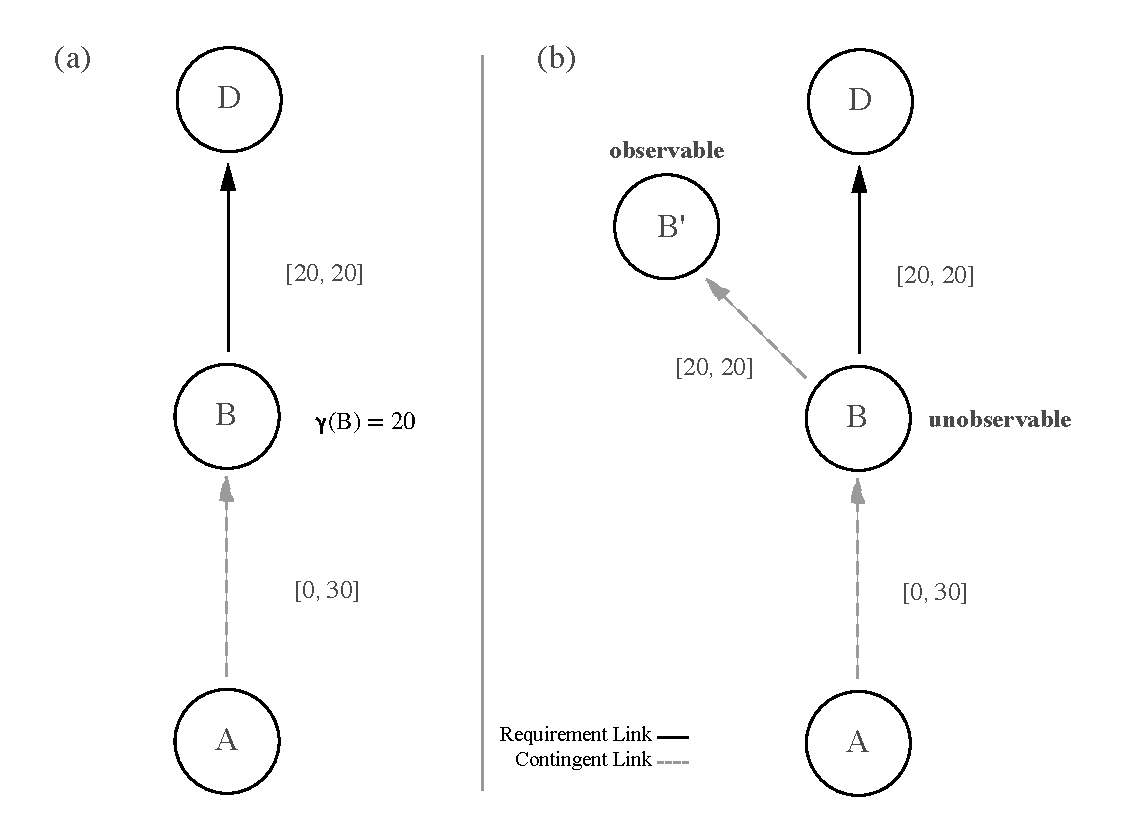
\includegraphics[width=0.75\textwidth]{POSTNU.pdf}
\end{figure}

It is not clear if controllability can be checked more efficiently across a greater subset of
POSTNUs beyond those without chained contingencies. However, it is worth highlighting that
variable-delay controllability can be leveraged to construct improved algorithms with respect to
scheduling and controllability of POSTNUs. The model for observation delay proposed by
variable-delay controllability can be expressed exactly as a POSTNU with a ``single-headed'' chained
contingency\footnote{To borrow the term ``single-headed'' from \citeprocitem{45}{[45]}.} as shown
in Figure \ref{fig:postnu}b; the main difference is that we represent the contingent link between \(B\) and
\(B'\) with our variable-delay function \(\gammabar(B)\). Hence, the algorithm we present for
variable-delay controllability can be used to both solve POSTNUs without chained contingencies, as
described above, as well as those POSTNUs with single-headed chained contingencies. Approaches
inspired by variable-delay controllability have been used to further expand POSTNU dynamic
controllability checking in more expressive chained instances \citeprocitem{45}{[45]}. We
hope that insights from variable-delay controllability will continue to expand the subset of POSTNUs
that can be controllability checked, and as such we advocate for continued development of the theory
of variable-delay controllability as a relevant framework for modelers.

%% This defines the bibliography file (main.bib) and the bibliography style.
%% If you want to create a bibliography file by hand, change the contents of
%% this file to a `thebibliography' environment.  For more information
%% see section 4.3 of the LaTeX manual.
\bibliography{extra-citations}
\begin{singlespace}
\begin{thebibliography}

\begin{hangparas}{1.5em}{1}
\hypertarget{citeproc_bib_item_1}{[1] N. Bhargava, C. Muise, and B. C. Williams, “Variable-delay controllability,” in \textit{IJCAI International Joint Conference on Artificial Intelligence}, 2018, vol. 2018-July, pp. 4660–4666. doi: \href{https://doi.org/10.24963/ijcai.2018/648}{10.24963/ijcai.2018/648}.\\}

\hypertarget{citeproc_bib_item_2}{[2] M. J. Miller, “Decision Support System Development For Human Extravehicular Activity,” Georgia Institute of Technology, 2017.\\}

\hypertarget{citeproc_bib_item_3}{[3] D. Wang and B. C. Williams, “TBurton: A divide and conquer temporal planner,” in \textit{Proceedings of the National Conference on Artificial Intelligence}, 2015, vol. 5, pp. 3409–3417.\\}

\hypertarget{citeproc_bib_item_4}{[4] J. W. McBarron, “Past, present, and future: The U.S. EVA Program,” \textit{Acta astronautica}, vol. 32, no. 1, pp. 5–14, 1994, doi: \href{https://doi.org/10.1016/0094-5765(94)90143-0}{10.1016/0094-5765(94)90143-0}.\\}

\hypertarget{citeproc_bib_item_5}{[5] C. P. Sonnett, “REPORT of the AD HOC WORKING GROUP ON APOLLO EXPERIMENTS AND TRAINING on the SCIENTIFIC ASPECTS OF THE APOLLO PROGRAM,” NASA, 1963.\\}

\hypertarget{citeproc_bib_item_6}{[6] J. M. Hurtado, K. Young, J. E. Bleacher, W. B. Garry, and J. W. Rice, “Field geologic observation and sample collection strategies for planetary surface exploration: Insights from the 2010 Desert RATS geologist crewmembers,” \textit{Acta astronautica}, vol. 90, no. 2, pp. 344–355, 2013, doi: \href{https://doi.org/10.1016/j.actaastro.2011.10.015}{10.1016/j.actaastro.2011.10.015}.\\}

\hypertarget{citeproc_bib_item_7}{[7] K. Young and T. Graff, “Planetary Science Context for EVA,” in \textit{NASA EVA Exploration Workshop}, 2020, p. 40.\\}

\hypertarget{citeproc_bib_item_8}{[8] A. Kanelakos, “Artemis EVA Flight Operations - Preparing for Lunar EVA Training \& Execution,” in \textit{NASA EVA Exploration Workshop}, 2020, p. 47.\\}

\hypertarget{citeproc_bib_item_9}{[9] C. Campbell, “Advanced EMU Portable Life Support System (PLSS) and Shuttle/ISS EMU Schematics, a Comparison,” \textit{42nd international conference on environmental systems}, pp. 1–18, 2012, doi: \href{https://doi.org/10.2514/6.2012-3411}{10.2514/6.2012-3411}.\\}

\hypertarget{citeproc_bib_item_10}{[10] E. S. Patterson and D. D. Woods, “Shift changes, updates, and the on-call architecture in space shuttle mission control,” \textit{Computer supported cooperative work}, vol. 10, no. 3-4, p. 27, 2001, doi: \href{https://doi.org/10.1023/A:1012705926828}{10.1023/A:1012705926828}.\\}

\hypertarget{citeproc_bib_item_11}{[11] S. J. Payler \textit{et al.}, “Developing Intra-EVA Science Support Team Practices for a Human Mission to Mars,” \textit{Astrobiology}, vol. 19, no. 3, pp. 387–400, 2019, doi: \href{https://doi.org/10.1089/ast.2018.1846}{10.1089/ast.2018.1846}.\\}

\hypertarget{citeproc_bib_item_12}{[12] D. A. Coan, “Exploration EVA System Concept of Operations Summary for Artemis Phase 1 Lunar Surface Mission,” NASA, Houston, TX, 2020.\\}

\hypertarget{citeproc_bib_item_13}{[13] M. A. Seibert, D. S. Lim, M. J. Miller, D. Santiago-Materese, and M. T. Downs, “Developing Future Deep-Space Telecommunication Architectures: A Historical Look at the Benefits of Analog Research on the Development of Solar System Internetworking for Future Human Spaceflight,” \textit{Astrobiology}, vol. 19, no. 3, pp. 462–477, Mar. 2019, doi: \href{https://doi.org/10.1089/ast.2018.1915}{10.1089/ast.2018.1915}.\\}

\hypertarget{citeproc_bib_item_14}{[14] M. J. Miller and K. M. Feigh, \textit{Addressing the envisioned world problem: A case study in human spaceflight operations}, vol. 5. Cambridge University Press, 2019. doi: \href{https://doi.org/10.1017/dsj.2019.2}{10.1017/dsj.2019.2}.\\}

\hypertarget{citeproc_bib_item_15}{[15] M. J. Miller, K. M. McGuire, and K. M. Feigh, “Information flow model of human extravehicular activity operations,” \textit{Ieee aerospace conference proceedings}, vol. 2015-June, 2015, doi: \href{https://doi.org/10.1109/AERO.2015.7118942}{10.1109/AERO.2015.7118942}.\\}

\hypertarget{citeproc_bib_item_16}{[16] M. J. Miller, K. M. McGuire, and K. M. Feigh, “Decision Support System Requirements Definition for Human Extravehicular Activity Based on Cognitive Work Analysis,” \textit{Journal of cognitive engineering and decision making}, vol. 11, no. 2, pp. 136–165, 2017, doi: \href{https://doi.org/10.1177/1555343416672112}{10.1177/1555343416672112}.\\}

NO\_ITEM\_DATA:Sehlke2019

\hypertarget{citeproc_bib_item_18}{[18] B. C. Williams, M. D. Ingham, S. H. Chung, and P. H. Elliott, “Model-based programming of intelligent embedded systems and robotic space explorers,” \textit{Proceedings of the ieee}, vol. 91, no. 1, pp. 212–236, 2003, doi: \href{https://doi.org/10.1109/JPROC.2002.805828}{10.1109/JPROC.2002.805828}.\\}

\hypertarget{citeproc_bib_item_19}{[19] B. C. Williams and R. J. Ragno, “Conflict-directed A* and its role in model-based embedded systems,” \textit{Discrete applied mathematics}, vol. 155, no. 12, pp. 1562–1595, 2007, doi: \href{https://doi.org/10.1016/j.dam.2005.10.022}{10.1016/j.dam.2005.10.022}.\\}

\hypertarget{citeproc_bib_item_20}{[20] R. E. Fikes and N. J. Nilsson, “Strips: A new approach to the application of theorem proving to problem solving,” \textit{Artificial intelligence}, vol. 2, no. 3-4, pp. 189–208, 1971, doi: \href{https://doi.org/10.1016/0004-3702(71)90010-5}{10.1016/0004-3702(71)90010-5}.\\}

\hypertarget{citeproc_bib_item_21}{[21] R. Dechter, I. Meiri, and J. Pearl, “Temporal constraint networks,” \textit{Artificial intelligence}, vol. 49, no. 1-3, pp. 61–95, 1991, doi: \href{https://doi.org/10.1016/0004-3702(91)90006-6}{10.1016/0004-3702(91)90006-6}.\\}

\hypertarget{citeproc_bib_item_22}{[22] E. Fernández González, “Generative Multi-Robot Task and Motion Planning Over Long Horizons,” Massachusetts Institute of Technology, 2018.\\}

\hypertarget{citeproc_bib_item_23}{[23] J. Chen, B. C. Williams, and C. Fan, “Optimal mixed discrete-continuous planning for linear hybrid systems,” in \textit{HSCC 2021 - Proceedings of the 24th International Conference on Hybrid Systems: Computation and Control (part of CPS-IoT Week)}, 2021, vol. 1. doi: \href{https://doi.org/10.1145/3447928.3456654}{10.1145/3447928.3456654}.\\}

\hypertarget{citeproc_bib_item_24}{[24] T. Vidal and H. Fargier, “Handling Contingency in Temporal Constraint Networks: From Consistency to Controllabilities,” \textit{Journal of experimental and theoretical artificial intelligence}, vol. 11, no. 1, pp. 23–45, 1999, doi: \href{https://doi.org/10.1080/095281399146607}{10.1080/095281399146607}.\\}

\hypertarget{citeproc_bib_item_25}{[25] P. H. Morris, N. Muscettola, and T. Vidal, “Dynamic Control Of Plans With Temporal Uncertainty,” 2001.\\}

\hypertarget{citeproc_bib_item_26}{[26] P. Morris and N. Muscettola, “Temporal dynamic controllability revisited,” \textit{Proceedings of the national conference on artificial intelligence}, vol. 3, pp. 1193–1198, 2005.\\}

\hypertarget{citeproc_bib_item_27}{[27] P. Morris, “A structural characterization of temporal dynamic controllability,” \textit{Lecture notes in computer science (including subseries lecture notes in artificial intelligence and lecture notes in bioinformatics)}, vol. 4204 LNCS, pp. 375–389, 2006, doi: \href{https://doi.org/10.1007/11889205_28}{10.1007/11889205\_28}.\\}

\hypertarget{citeproc_bib_item_28}{[28] P. Morris, “Dynamic controllability and dispatchability relationships,” \textit{Lecture notes in computer science (including subseries lecture notes in artificial intelligence and lecture notes in bioinformatics)}, vol. 8451 LNCS, no. Dc, pp. 464–479, 2014, doi: \href{https://doi.org/10.1007/978-3-319-07046-9_33}{10.1007/978-3-319-07046-9\_33}.\\}

\hypertarget{citeproc_bib_item_29}{[29] A. Cimatti, A. Micheli, and M. Roveri, “Solving temporal problems with uncertainty using SMT: Strong Controllability,” \textit{Constraints}, vol. 20, no. 1, pp. 1–29, 2012, doi: \href{https://doi.org/10.1007/s10601-014-9167-5}{10.1007/s10601-014-9167-5}.\\}

\hypertarget{citeproc_bib_item_30}{[30] M. Ingham, R. Ragno, A. Wehowsky, and B. Williams, “The Reactive Model-based Programming Language,” MIT Space Systems and Artificial Intelligence Laboratories, 2002.\\}

\hypertarget{citeproc_bib_item_31}{[31] N. Bhargava, “Multi-Agent Coordination under Limited Communication,” Massachusetts Institute of Technology, 2020.\\}

\hypertarget{citeproc_bib_item_32}{[32] M. D. Moffitt, “On the partial observability of temporal uncertainty,” \textit{Proceedings of the national conference on artificial intelligence}, vol. 2, pp. 1031–1037, 2007.\\}

\hypertarget{citeproc_bib_item_33}{[33] G. Kiczales, J. Des Rivières, and D. G. Bobrow, \textit{The art of the metaobject protocol}. Cambridge, Mass: MIT Press, 1991.\\}

\hypertarget{citeproc_bib_item_34}{[34] M. Fox and D. Long, “PDDL2.1: An extension to PDDL for expressing temporal planning domains,” \textit{Journal of artificial intelligence research}, vol. 20, pp. 61–124, 2003, doi: \href{https://doi.org/10.1613/jair.1129}{10.1613/jair.1129}.\\}

\hypertarget{citeproc_bib_item_35}{[35] N. Bhargava, C. Muise, T. Vaquero, and B. Williams, “Delay Controllability : Multi-Agent Coordination under Communication Delay,” Massachusetts Institute of Technology, Cambridge, MA, 2018.\\}

\hypertarget{citeproc_bib_item_36}{[36] L. Hunsberger, “Efficient execution of dynamically controllable simple temporal networks with uncertainty,” \textit{Acta informatica}, vol. 53, no. 2, pp. 89–147, 2016, doi: \href{https://doi.org/10.1007/s00236-015-0227-0}{10.1007/s00236-015-0227-0}.\\}

\hypertarget{citeproc_bib_item_37}{[37] N. Bhargava, C. Muise, T. Vaquero, and B. Williams, “Managing communication costs under temporal uncertainty,” in \textit{IJCAI International Joint Conference on Artificial Intelligence}, 2018, vol. 2018-July, pp. 84–90. doi: \href{https://doi.org/10.24963/ijcai.2018/12}{10.24963/ijcai.2018/12}.\\}

\hypertarget{citeproc_bib_item_38}{[38] L. Hunsberger, “A faster execution algorithm for dynamically controllable STNUs,” \textit{Proceedings of the 20th international symposium on temporal representation and reasoning}, pp. 26–33, 2013, doi: \href{https://doi.org/10.1109/TIME.2013.13}{10.1109/TIME.2013.13}.\\}

\hypertarget{citeproc_bib_item_39}{[39] L. Hunsberger, “Fixing the semantics for dynamic controllability and providing a more practical characterization of dynamic execution strategies,” \textit{Time 2009 - 16th international symposium on temporal representation and reasoning}, pp. 155–162, 2009, doi: \href{https://doi.org/10.1109/TIME.2009.25}{10.1109/TIME.2009.25}.\\}

\hypertarget{citeproc_bib_item_40}{[40] G. Casanova, C. Pralet, C. Lesire, and T. Vidal, “Solving dynamic controllability problem of multi-agent plans with uncertainty using mixed integer linear programming,” \textit{Frontiers in artificial intelligence and applications}, vol. 285, pp. 930–938, 2016, doi: \href{https://doi.org/10.3233/978-1-61499-672-9-930}{10.3233/978-1-61499-672-9-930}.\\}

\hypertarget{citeproc_bib_item_41}{[41] J. L. Stedl, “Managing Temporal Uncertainty Under Limited Communication: A Formal Model of Tight and Loose Team Coordination,” Massachusetts Institute of Technology, 2004.\\}

\hypertarget{citeproc_bib_item_42}{[42] L. Lamport \textit{et al.}, “The Part-Time Parliment,” \textit{Acm transactions on computer systems}, vol. 16, no. 2, pp. 373–386, 1998, doi: \href{https://doi.org/10.1145/568425.568433}{10.1145/568425.568433}.\\}

\hypertarget{citeproc_bib_item_43}{[43] D. Ongaro and J. Ousterhout, “In search of an understandable consensus algorithm,” \textit{Proceedings of the 2014 usenix annual technical conference, usenix atc 2014}, pp. 305–319, 2014.\\}

\hypertarget{citeproc_bib_item_44}{[44] A. Bit-Monnot, M. Ghallab, and F. Ingrand, “Which contingent events to observe for the dynamic controllability of a plan,” \textit{Ijcai international joint conference on artificial intelligence}, vol. IJCAI-16, no. July, pp. 3038–3044, 2016.\\}

\hypertarget{citeproc_bib_item_45}{[45] P. H. Morris and A. Bit-monnot, “Dynamic Controllability with Single and Multiple Indirect Observations,” in \textit{ICAPS 2019 - Proceedings of the 29th International Conference on Automated Planning and Scheduling}, 2019, p. 9.\\}\bigskip
\end{hangparas}

\end{thebibliography}
\end{singlespace}
\end{document}
\end{document}